%\wip{Text to be updated to reflect ATLAS+CMS combination.}
%\newpage
The projections documented in this section~\cite{CMS-PAS-FTR-18-011,ATL-PHYS-PUB-2018-054} are based on the extrapolation of the following analyses:

\begin{itemize}
	\item \hgg, with $\ggh$, $\vbf$, $\vh$ and $\tth$ production~\cite{Sirunyan:2018ouh,ATLAS-CONF-2018-028,Aaboud:2018urx},
	\item \hzzllll, with $\ggh$, $\vbf$, $\vh$ and $\tth$ production~\cite{HIG16041,ATLAS-CONF-2018-018},
	\item \hwwlnln, with $\ggh$, $\vbf$ and $\vh$ production~\cite{HIG-16-042,Aaboud:2018jqu},
	\item \htt, with $\ggh$ and $\vbf$ production~\cite{HIG16043,ATLAS-CONF-2018-021},
	\item \vh production with \hbb decay~\cite{HIG16044,Aaboud:2018zhk},
	\item Boosted H production with \hbb~ decay~\cite{HIG17010},
	\item \tth production with \hlep~\cite{Sirunyan:2018shy,Aaboud:2017jvq},
	\item \tth production with \hbb~\cite{bib:hig-17-026,Sirunyan:2018ygk,Aaboud:2017rss},
	\item \hmm, with $\ggh$ and $\vbf$ production~\cite{HIG-17-019,ATLAS-CONF-2018-026},
	\item \hzg, with \ggh and \vbf production~\cite{Aaboud:2017uhw}.
\end{itemize}

The projected results given in this section are based on the combined measurement of these channels~\cite{Sirunyan:2018koj,ATLAS-CONF-2018-031}. In the following results, the signal model in the $\hmm$ channel is modified to account for the improved di-muon mass resolution in the Phase-2 ATLAS and CMS tracker upgrades~\cite{Klein:2017nke,Collaboration:2285585}. In CMS, it is estimated that the reduced material budget and improved spatial resolution of the upgraded tracker will yield a $40\%$ improvement in the di-muon mass resolution, for example a reduction from $1.1\%$ to $0.65\%$ for muons in the barrel region. In ATLAS, instead, the reduction of the di-muon invariant mass resolution is estimated to be between 15\% and 30\% depending on the analysis categories (forward/central).

In the ATLAS projection the expected signal and background yields in all channels are scaled to account for the increasing cross sections going from $\sqrt{s}=13\TeV$ to $\sqrt{s}=14\TeV$, while no scaling is performed in the CMS projection. The impact of this scaling on the projected sensitivity is found to be small.

% The results in this section are presented under the two systematic uncertainty scenarios S1 and S2 as described in Section~\ref{sec:extrap}.

%\wip{Switch to cross section and branching ratio results without inclusive theory uncertainties.}
%Projections are given for two parametrisations of the signal, based on signal strength modifiers $\mu$, defined as the ratio between the measured Higgs boson yield and its SM expectation. One set of parameters $\mu^{f}$, where $f = \zz$, $\ww$, $\hgg$, $\tautau$, $\bb$ and $\mumu$, are introduced to scale the branching fractions of each decay mode independently, assuming the SM cross sections for the production modes. Another set, $\mu_{i}$, where $i=\ggh$, $\vbf$, $\wh$, $\zh$ and $\tth$, scale each production cross section independently, assuming the SM values of the branching fractions.

%%%updated - with cross sections , adding xs per decay mode %%
Projections are given for three different sets of measurements:
\begin{itemize}
    \item \textbf{Higgs boson production cross sections in different decay channels}: the parameters of interest are the cross sections times branching fractions for ggH, VBF, WH, ZH and ttH production in each relevant decay mode, normalised to their SM predictions.
    \item \textbf{Higgs boson production cross sections}:  the parameters of interest are the production cross sections normalised to the corresponding SM predictions  $\sigma_{i}/\sigma_{i}^{\mathrm{SM}}$  where $i=\ggh$, $\vbf$, $\wh$, $\zh$ and $\tth$, assuming the SM values for the branching fractions. The small contribution from bbH is grouped with \ggh while the \zh process includes \zh production with the gluon-gluon initial state. The overall theoretical uncertainties on the inclusive SM cross section predictions are not included, while the uncertainties on the branching ratios are included as the values are assumed to be given by the SM.
    \item \textbf{Higgs boson branching fractions}: the parameters of interest are the branching fractions normalised to the corresponding SM values $\BR_{f}/\BR_{f}^{\mathrm{SM}}$, where $f = \zz$, $\ww$, $\PGg\PGg$, $\tautau$, $\bb$, $\mumu$, $\PZ\PGg$ assuming the SM cross sections for the production modes. In this case  the uncertainties on the decay branching ratios are not included, while the overall QCD scales and PDF+$\alpha_{S}$ uncertainties on the inclusive production cross sections are included.

\end{itemize}

For each projected measurement the uncertainty is decomposed into four components: statistical, experimental, background theory and signal theory.
The combination is based on the assumption that these components are independent within each experiment. Among them, the statistical and experimental uncertainties are treated as fully uncorrelated between the two experiments, while the signal and background theory uncertainties are assumed to be fully correlated. The combination is performed for each parameter individually using the the BLUE methodology as described in Ref.~\cite{Valassi:2003mu}. This procedure does not take into account correlations that may exist between parameters. These arise when analysis channels are sensitive to more than one production or decay mode and the chosen fit observables do not fully distinguish between these, as well as when the same systematic uncertainties apply to multiple production or decay modes. The effect of including these correlations via a simultaneous combination of all parameters has been verified, utilising the same BLUE methodology and including the complete covariance matrices for both experiments, and is found to have a minor effect on the projection results. Specifically, the effect on the combined statistical and experimental uncertainties is negligible given the reported precision. For the theory uncertainties this procedure can lead to smaller values than in the case where these correlations are neglected. This is a feature of the methodology of Ref.~\cite{Valassi:2003mu}, due to the different approaches concerning the theoretical uncertainties used in the extrapolations by the two experiments, which leads to differences in some of the correlation values. However, it is expected that by the time of the HL-LHC both experiments will employ a more consistent treatment of the theoretical uncertainties, making this reduction largely artificial. This motivates the choice to combine measurement projections independently and neglect such correlations in the following results.

% In addition, correlations may arise when the same systematic uncertainties apply to multiple production or decay modes.
%An important aspect of the projected measurements is how the correlations between the measured parameters are expected to evolve. Correlations arise when analysis channels are sensitive to more than one production or decay mode and the chosen fit observables do not fully distinguish between these. 
% In addition, correlations may arise when the same systematic uncertainties apply to multiple production or decay modes.


% In the ATLAS-CMS combination of each set of measurements  described before, all the quantities are combined at the same time, making use of the complete covariance matrix of the ATLAS and CMS input projections and thus taking into account all correlations between them, using the BLUE methodology as described in Ref.~\cite{Valassi:2003mu}. This is particularly important for the BR measurements, where the theoretical uncertainties on the SM predictions for the per-production-mode cross sections are taken into account introducing non-negligible correlation among the branching ratios, as well as for the results given for the parametrisations based on the coupling modifier presented in Section~\ref{sec2:exp_kappa}.
% Due to the different approaches concerning the theoretical uncertainties used in the extrapolations by the two experiments, the covariance matrix for the theoretical uncertainties of the various set of measurements looks  different between ATLAS (smaller correlations) and CMS (larger correlations) . As a result of this difference, when combining with the methodology of Ref.~\cite{Valassi:2003mu}, a smaller uncertainty is obtained compared to the case when the correlation among the measurements are not taken into account. 
%\wip{to add few words on how the ATLAS-CMS combination is performed}


%-------------------------------------------------------------

\subsubsection{Production mode cross-sections in different decay channels}
\label{sec:expcomb_prodtimesdecay}
The expected $\pm 1\sigma$ uncertainties on the production mode cross sections in the different decay channels in S2 are summarised in Figure~\ref{fig:summary_A1_5PD_ggH_VBF} for \ggh and \vbf, in Figure~\ref{fig:summary_A1_5PD_WH_ZH} for \wh and \zh, in Figure~\ref{fig:summary_A1_5PD_ttH}. These are shown for ATLAS, CMS and their combination. Additionally, the numerical values for the ATLAS-CMS combination in scenario S2 are also reported in the figures, with the uncertainty decomposed in three components: statistical, experimental and theory.
There are few cases where the extrapolation is currently available only for one experiment (e.g. only $gg \rightarrow H \rightarrow bb$ in CMS, and only \hzg in ATLAS). In these cases, the combined result is obtained by using the same available extrapolation  for both experiments.
The correlations between the different production mode cross-sections in different decay channels are in general small, with the exception of the \zh and \wh measurements in the \hzz decay (for this reason the \vh cross-section is also reported) and the \ggh and \vbf production mode cross sections in the \hmm decay. 

%%\wip{to add few consideration on the combined results for the dominant unc. components}
%% Maria: commented out 29/Jan

%Since in the current \hzzllll ATLAS projection there is a strongly anti-correlation between \wh and \zh measurements, also the \vh cross-section is reported. 
The numerical values of the expected $\pm 1\sigma$ uncertainties on the per-production-mode cross sections in the different decay channels for the ATLAS and CMS projections are given in Table~\ref{tab:summary_A1_5PD}. The table  gives the breakdown of the uncertainty into four components: statistical, signal theory, background theory and experimental for both scenarios S1 and S2. 


\begin{figure}[hbtp]
\centering
%width=0.48\textwidth
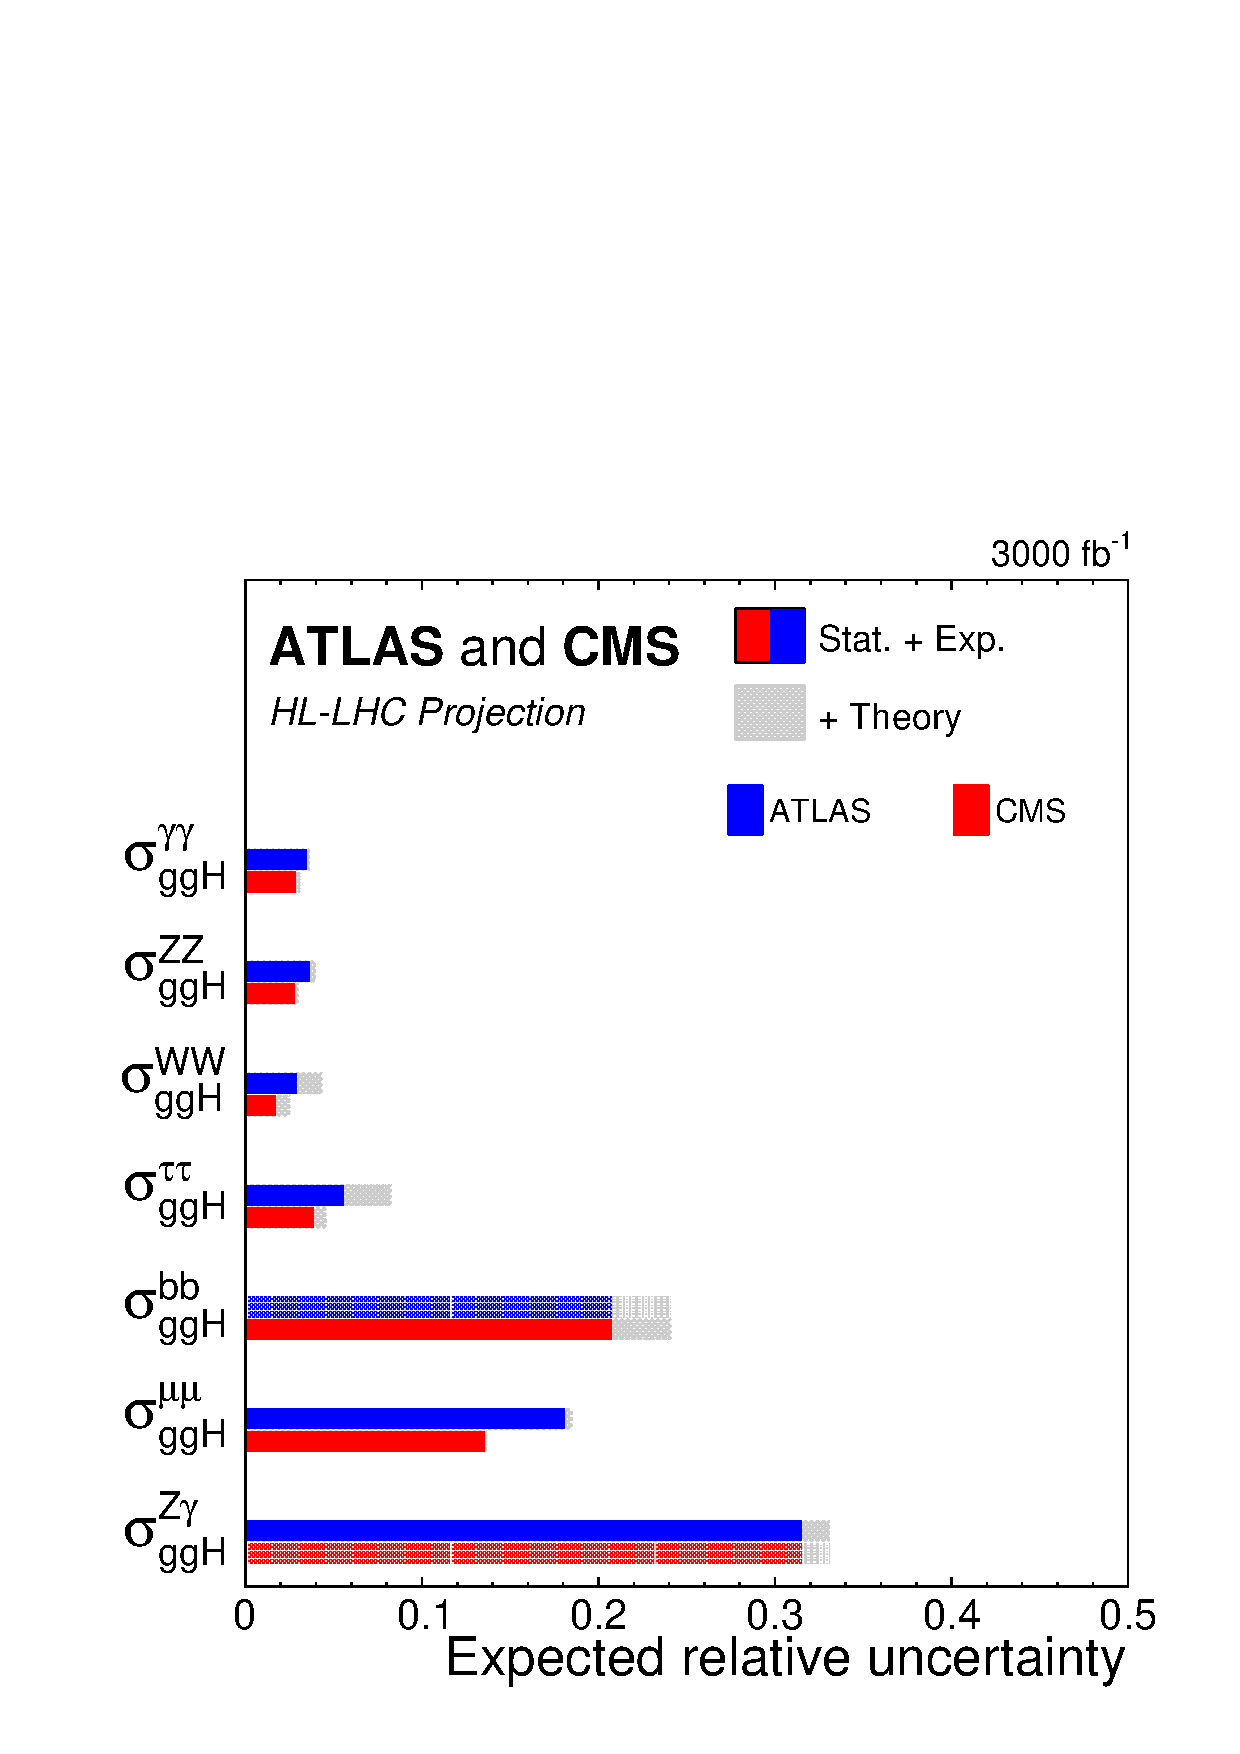
\includegraphics[height=0.332\textheight]{\main/section2/plots/comb/yr_combined_summary_A1_5PD_3000_ggH.pdf}%
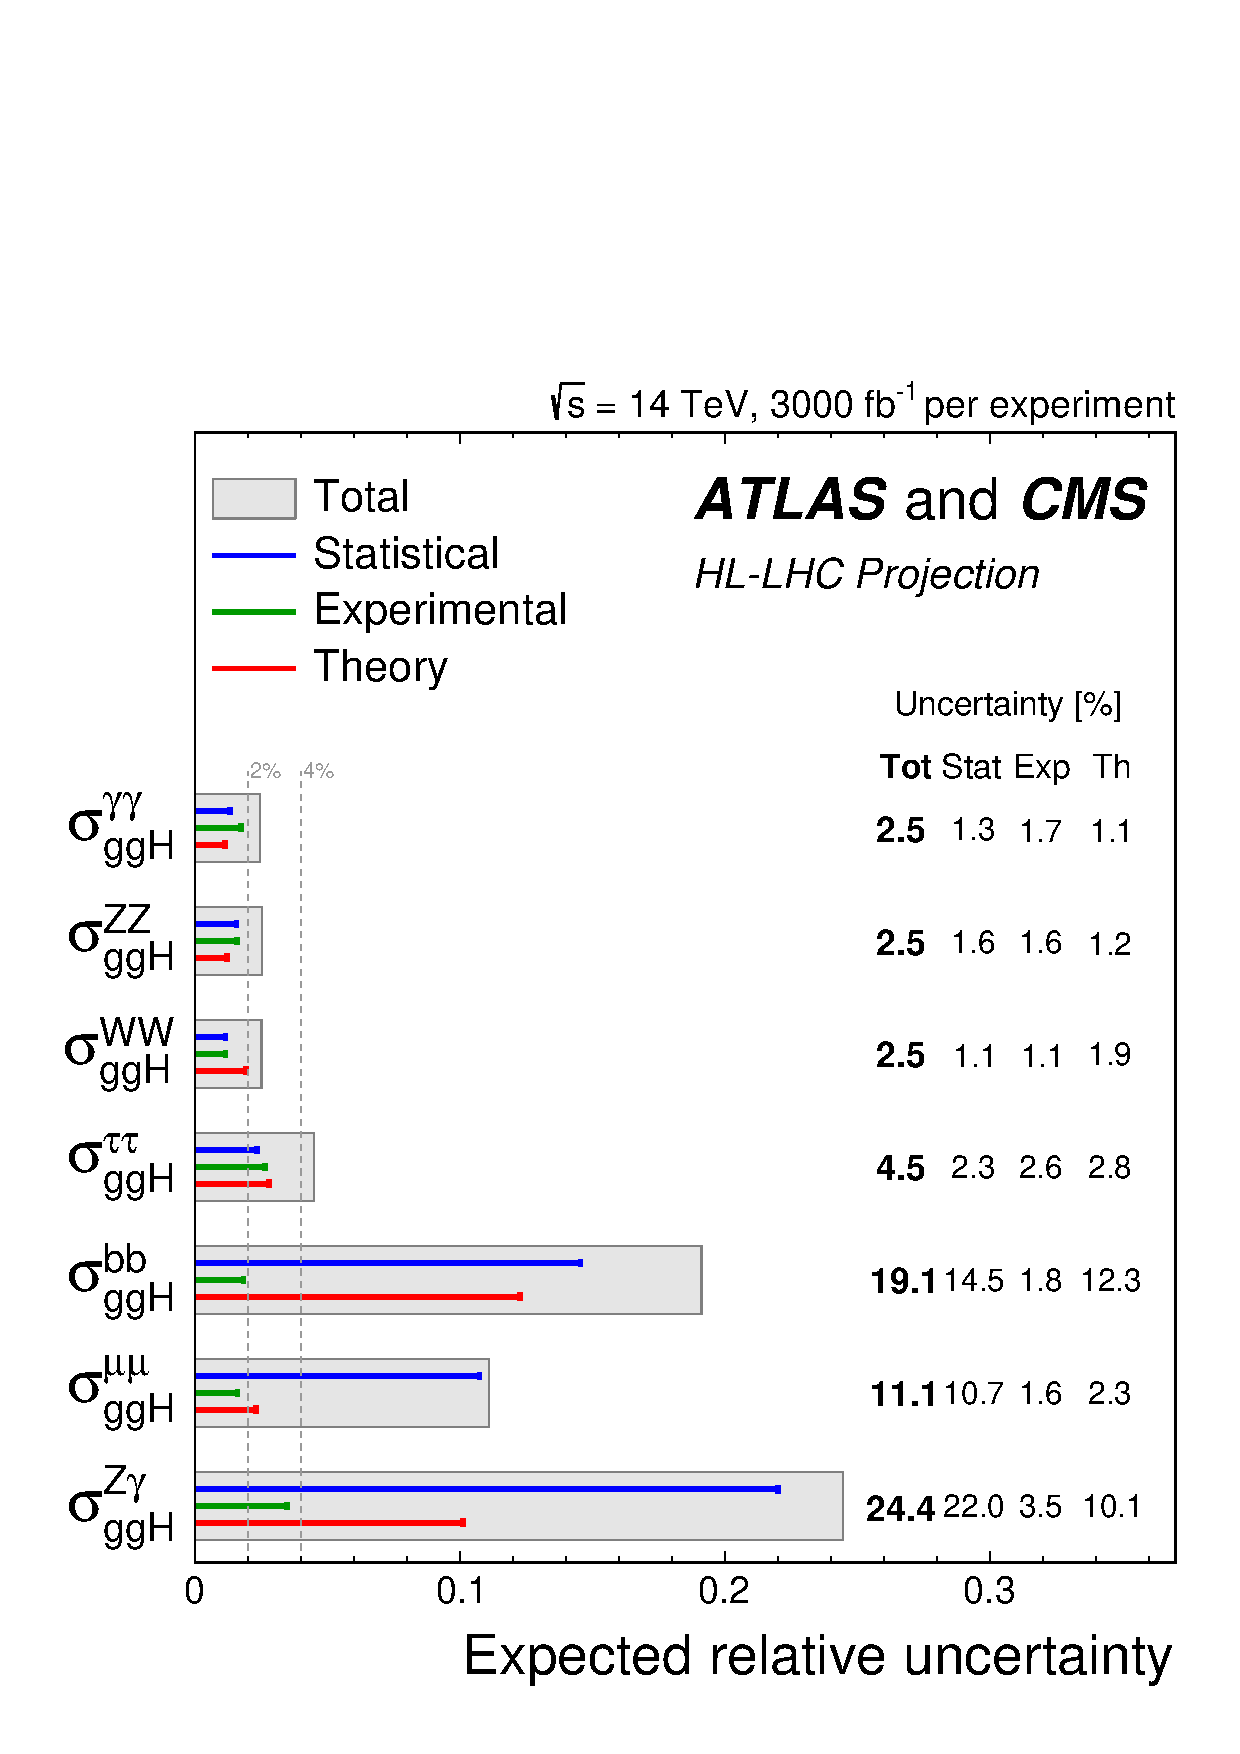
\includegraphics[height=0.33\textheight]{\main/section2/plots/comb/yr_combined_5PD_ggH.pdf}\\
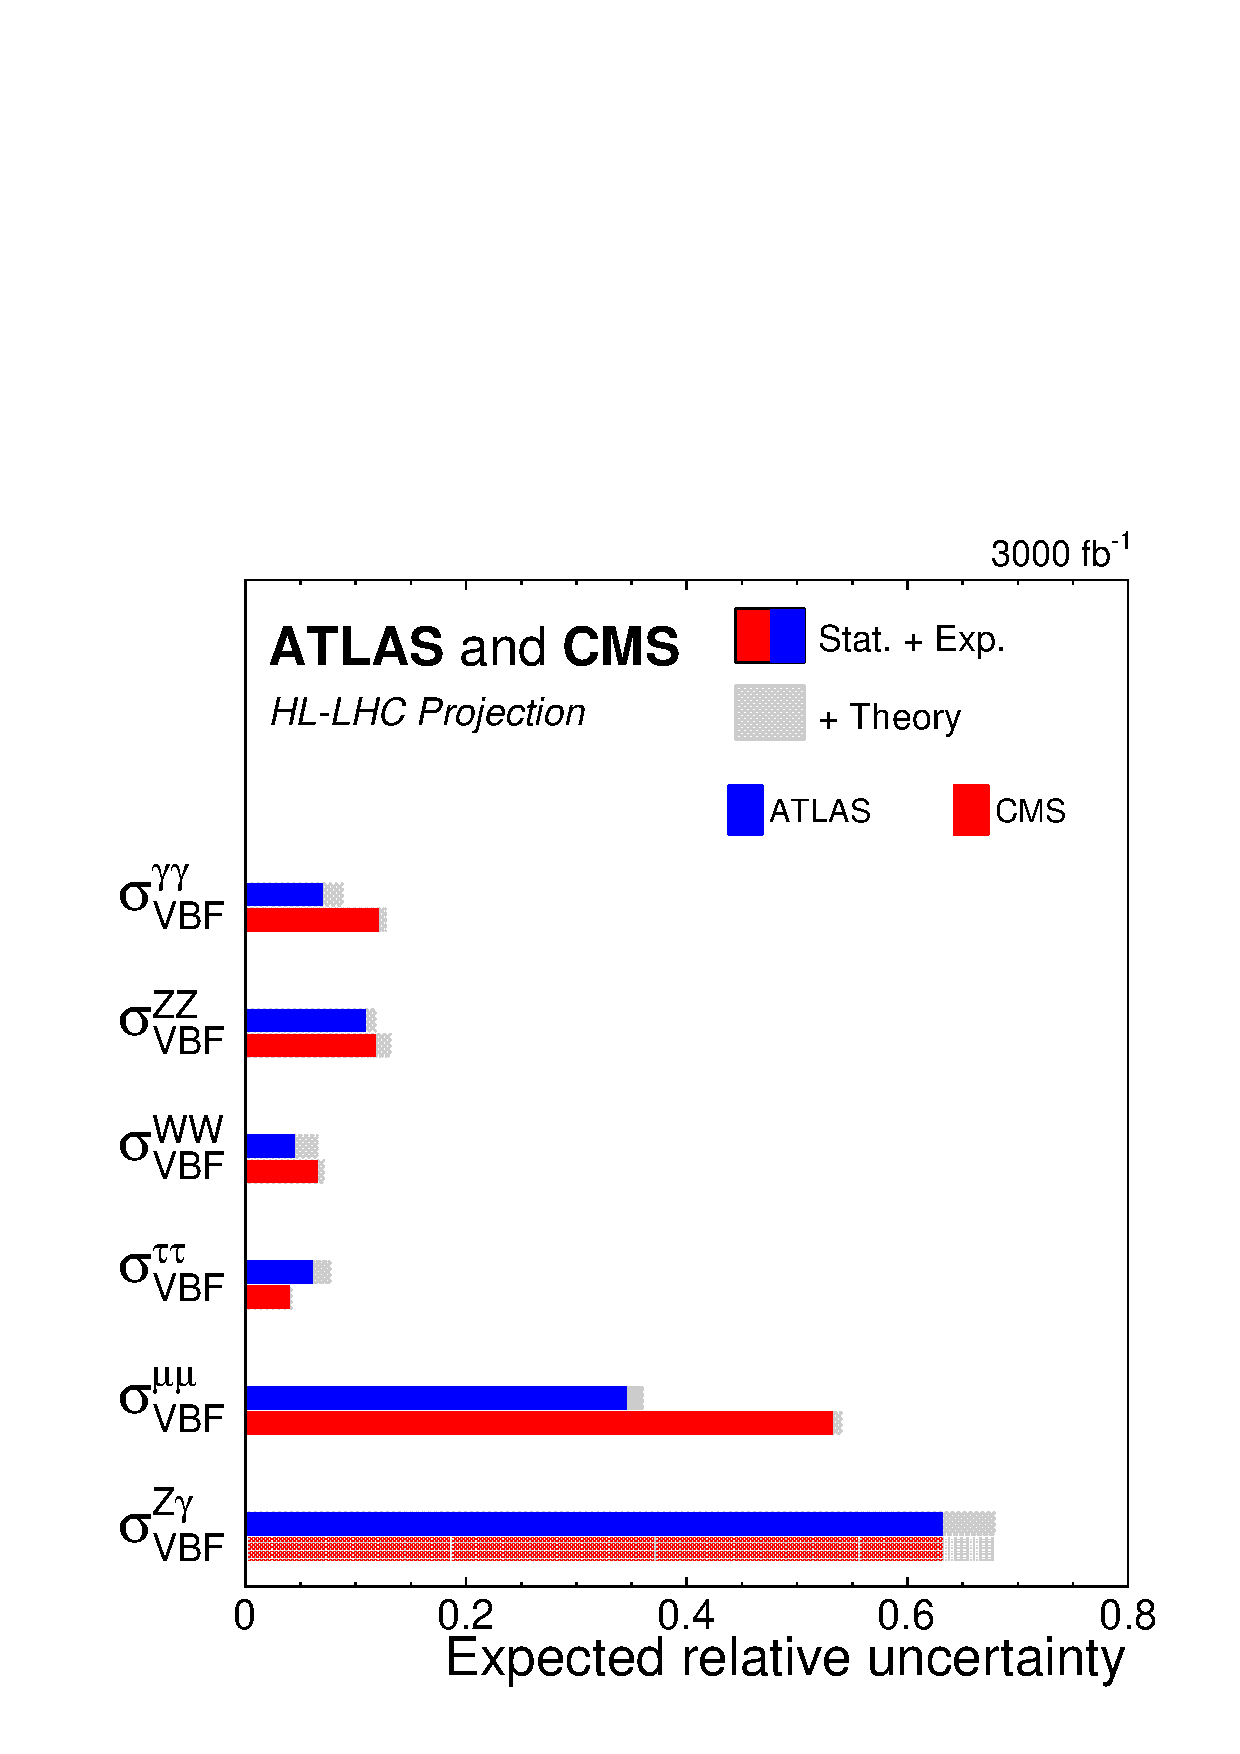
\includegraphics[height=0.332\textheight]{\main/section2/plots/comb/yr_combined_summary_A1_5PD_3000_VBF.pdf}%
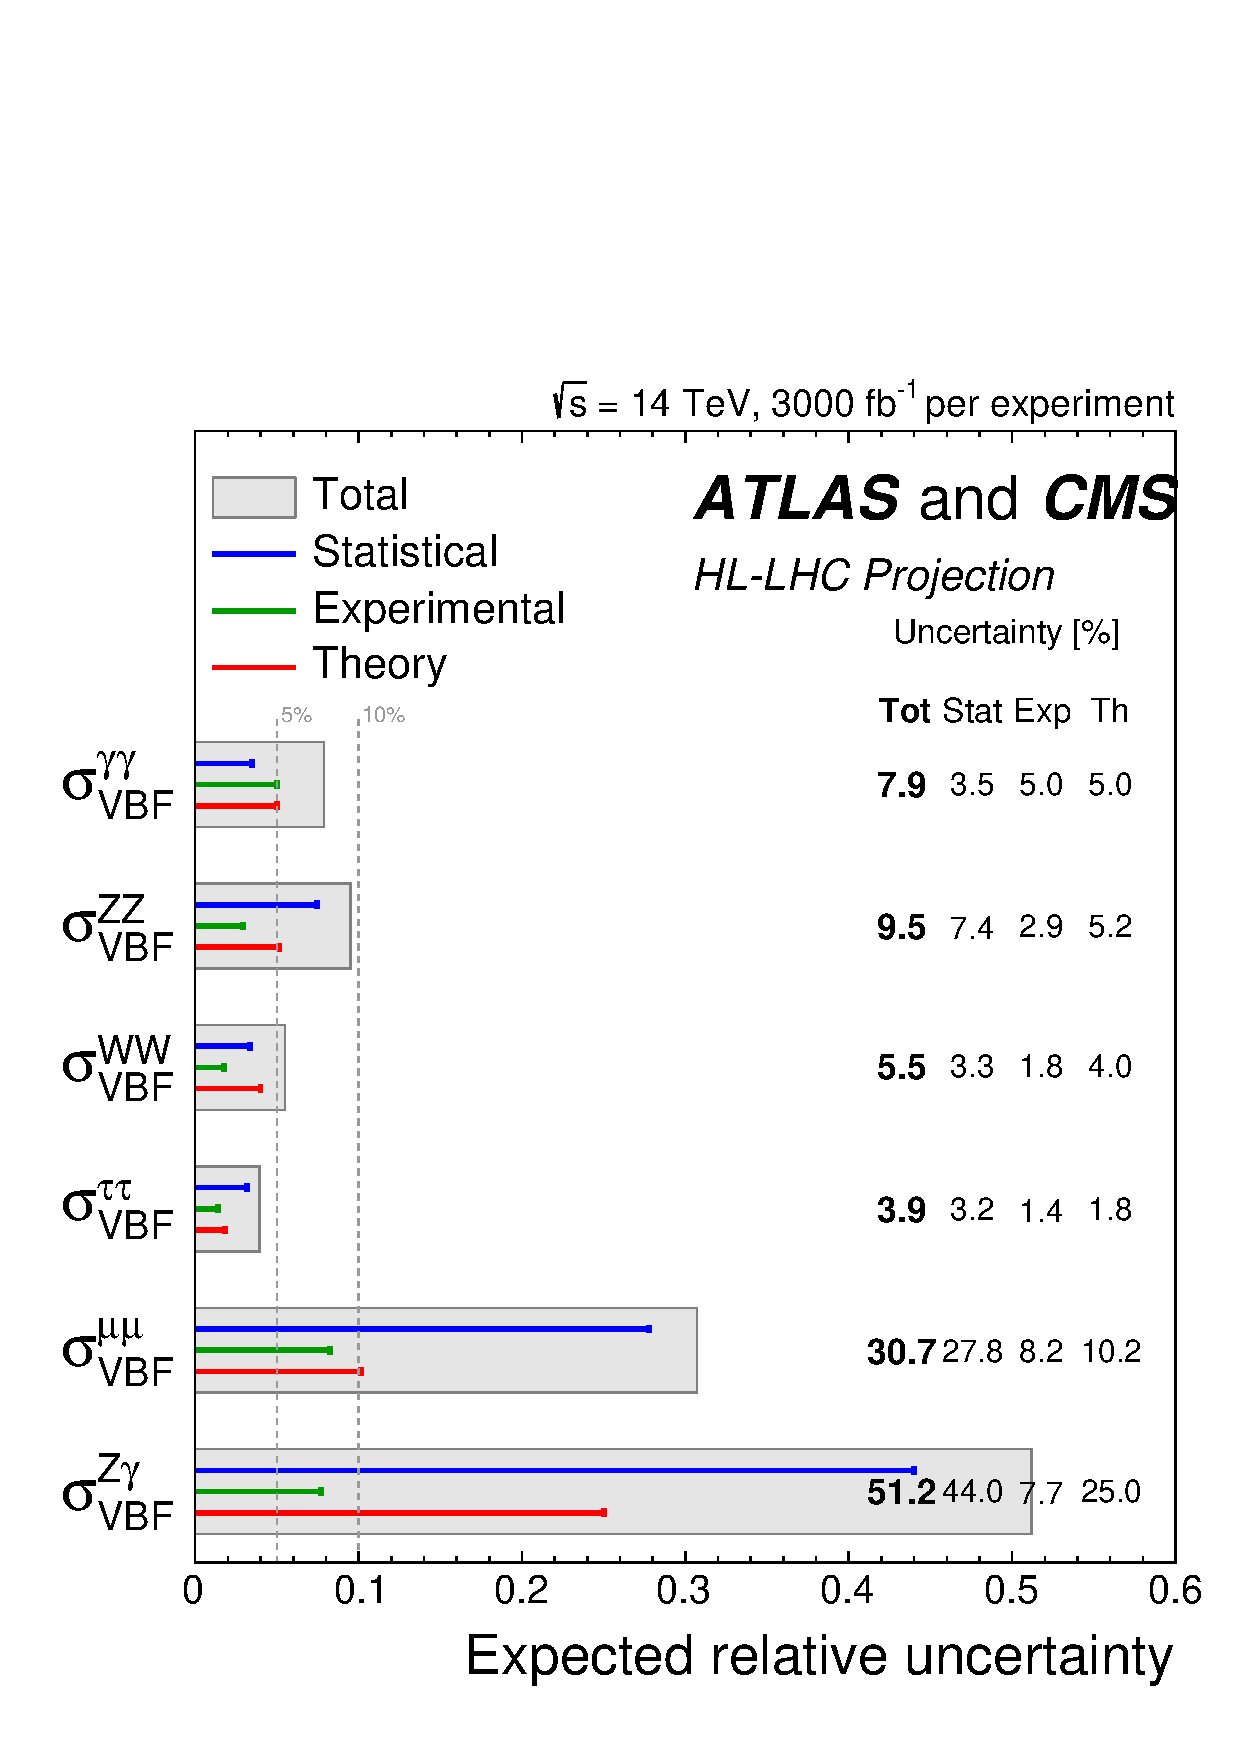
\includegraphics[height=0.33\textheight]{\main/section2/plots/comb/yr_combined_5PD_VBF.pdf}%
\caption{(left) Summary plot showing the total expected $\pm 1\sigma$ uncertainties in S2 (with YR18 systematic uncertainties) on the \ggh (top) and \vbf (bottom) production cross sections in the different decay modes normalised to the SM predictions   for ATLAS(blue)  and CMS (red). The filled coloured box corresponds to the statistical and experimental systematic uncertainties, while the hatched grey area represent the additional contribution to the total uncertainty due to theoretical systematic uncertainties. In the cases where  the extrapolation is performed only by one experiment, same performances are assumed for the other experiment and this is indicated by a  hatched bar.
(right) Summary plot showing the total expected $\pm 1\sigma$  uncertainties in S2 (with YR18 systematic uncertainties) on the \ggh (top) and \vbf (bottom) production cross sections in the different decay modes normalised to the SM predictions for the combination of ATLAS and CMS extrapolations. For each measurement,  the total uncertainty is indicated by a grey box while the statistical, experimental and theory uncertainties are indicated by a blue, green and red line respectively. In addition, the numerical values are also reported.}
\label{fig:summary_A1_5PD_ggH_VBF}
\end{figure}


\begin{figure}[hbtp]
\centering
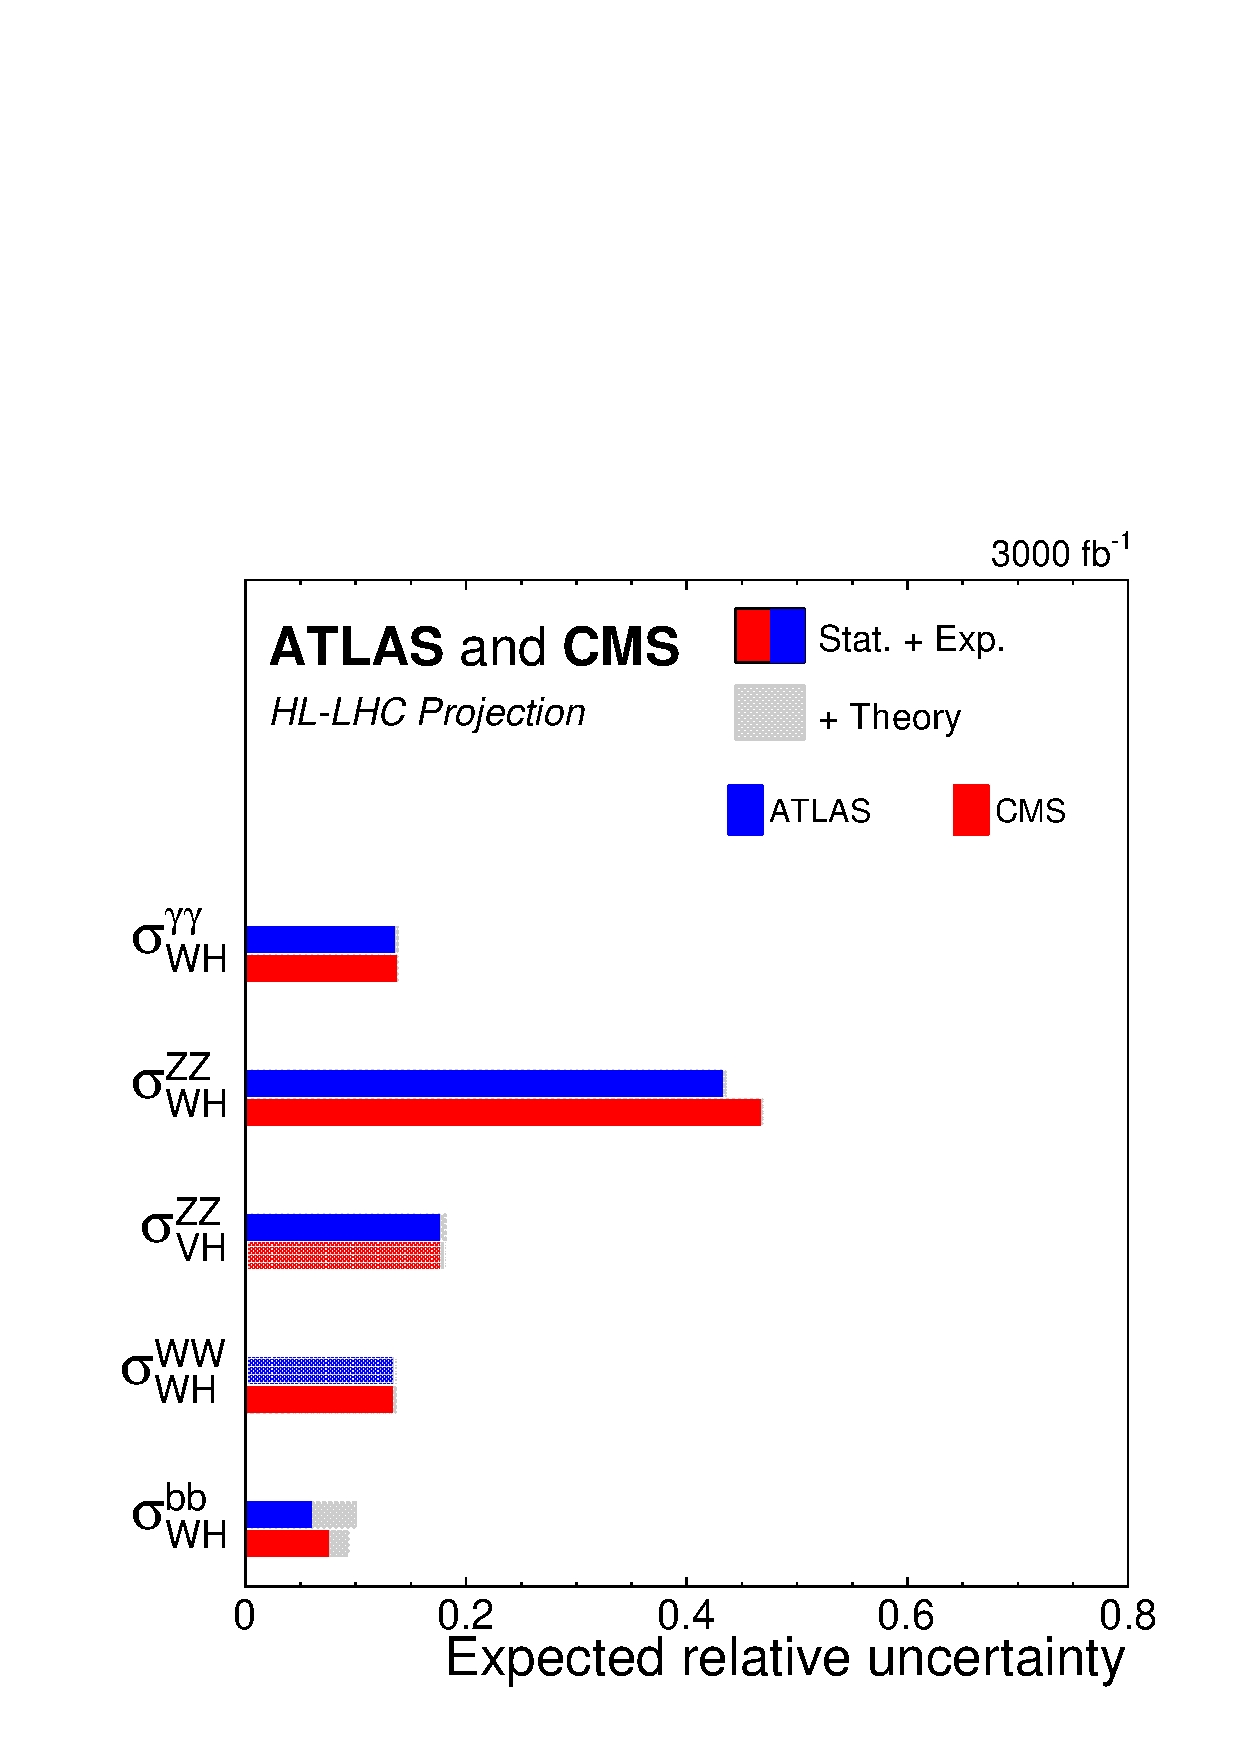
\includegraphics[height=0.332\textheight]{\main/section2/plots/comb/yr_combined_summary_A1_5PD_3000_WH.pdf}%
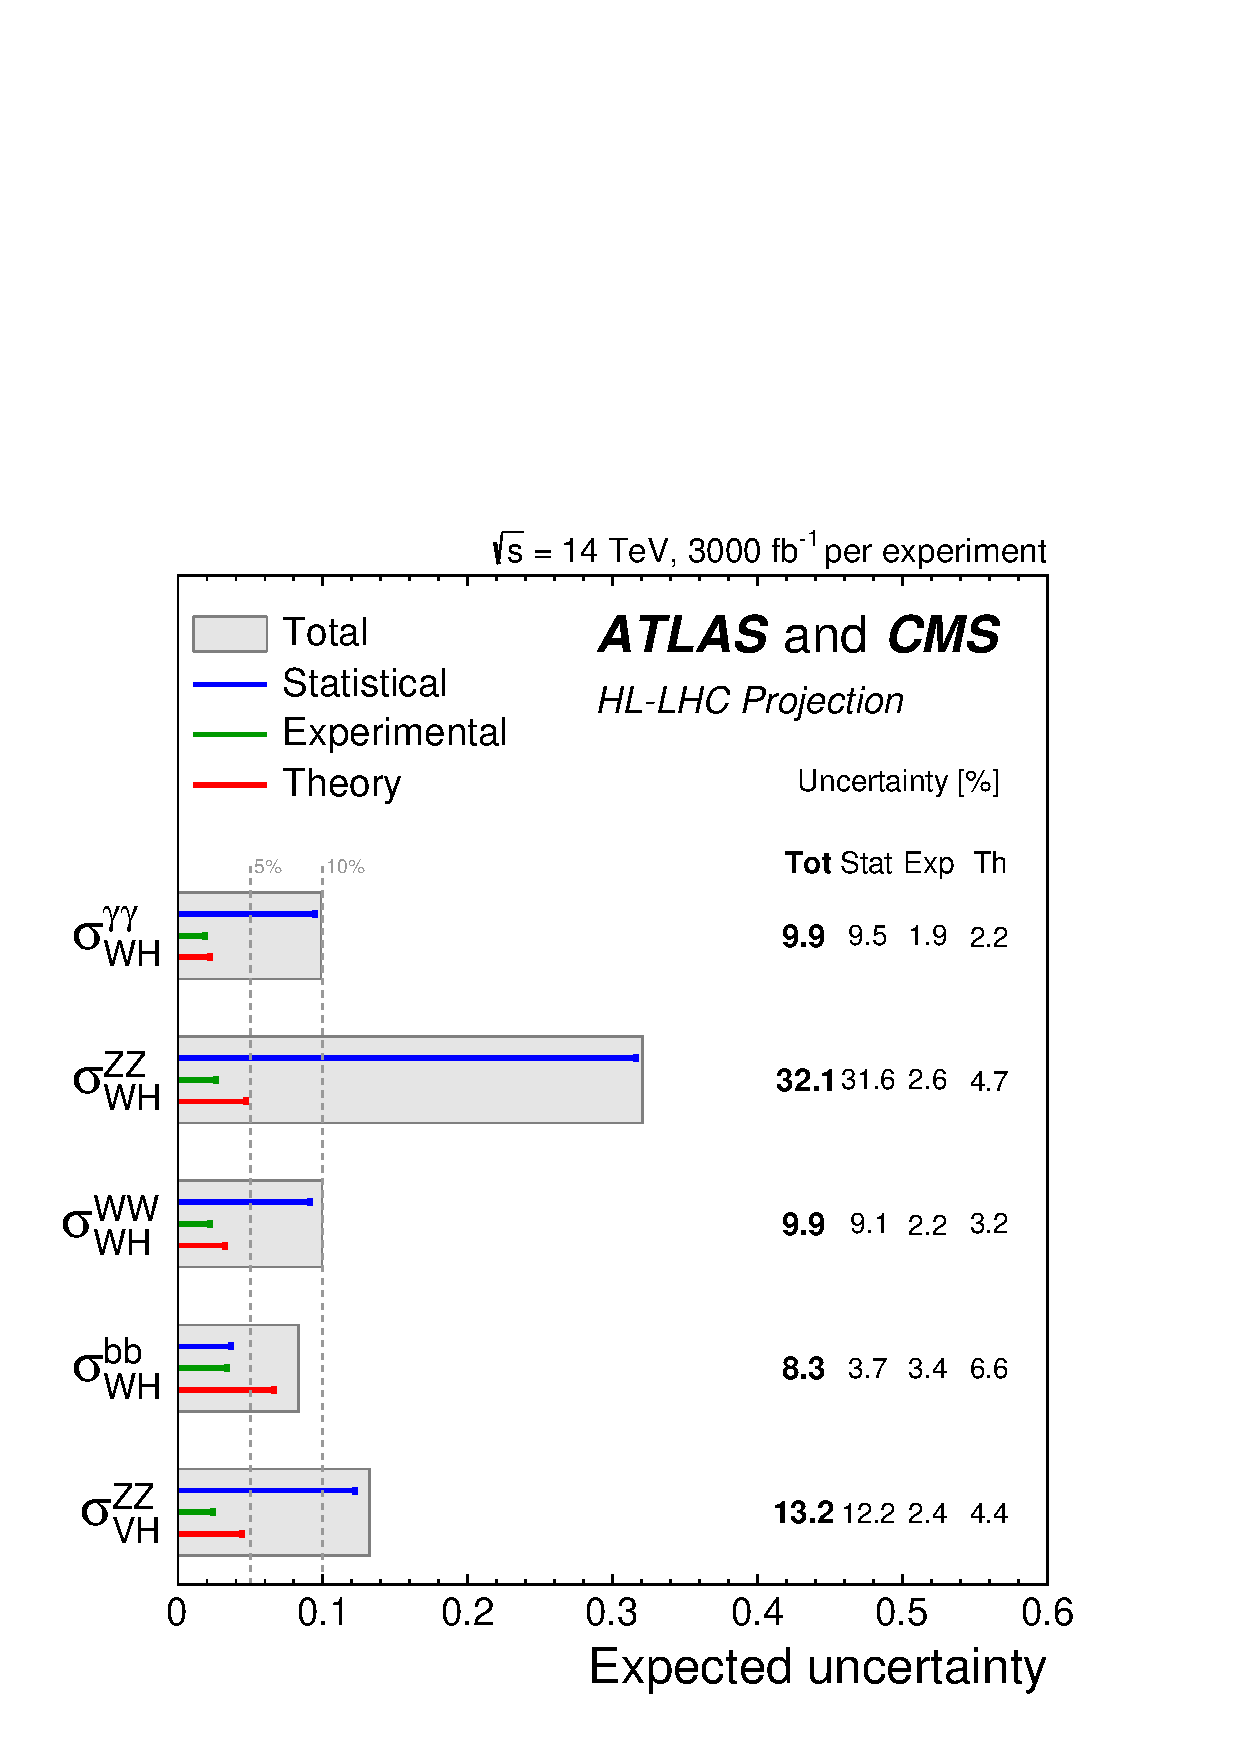
\includegraphics[height=0.33\textheight]{\main/section2/plots/comb/yr_combined_5PD_WH.pdf}\\
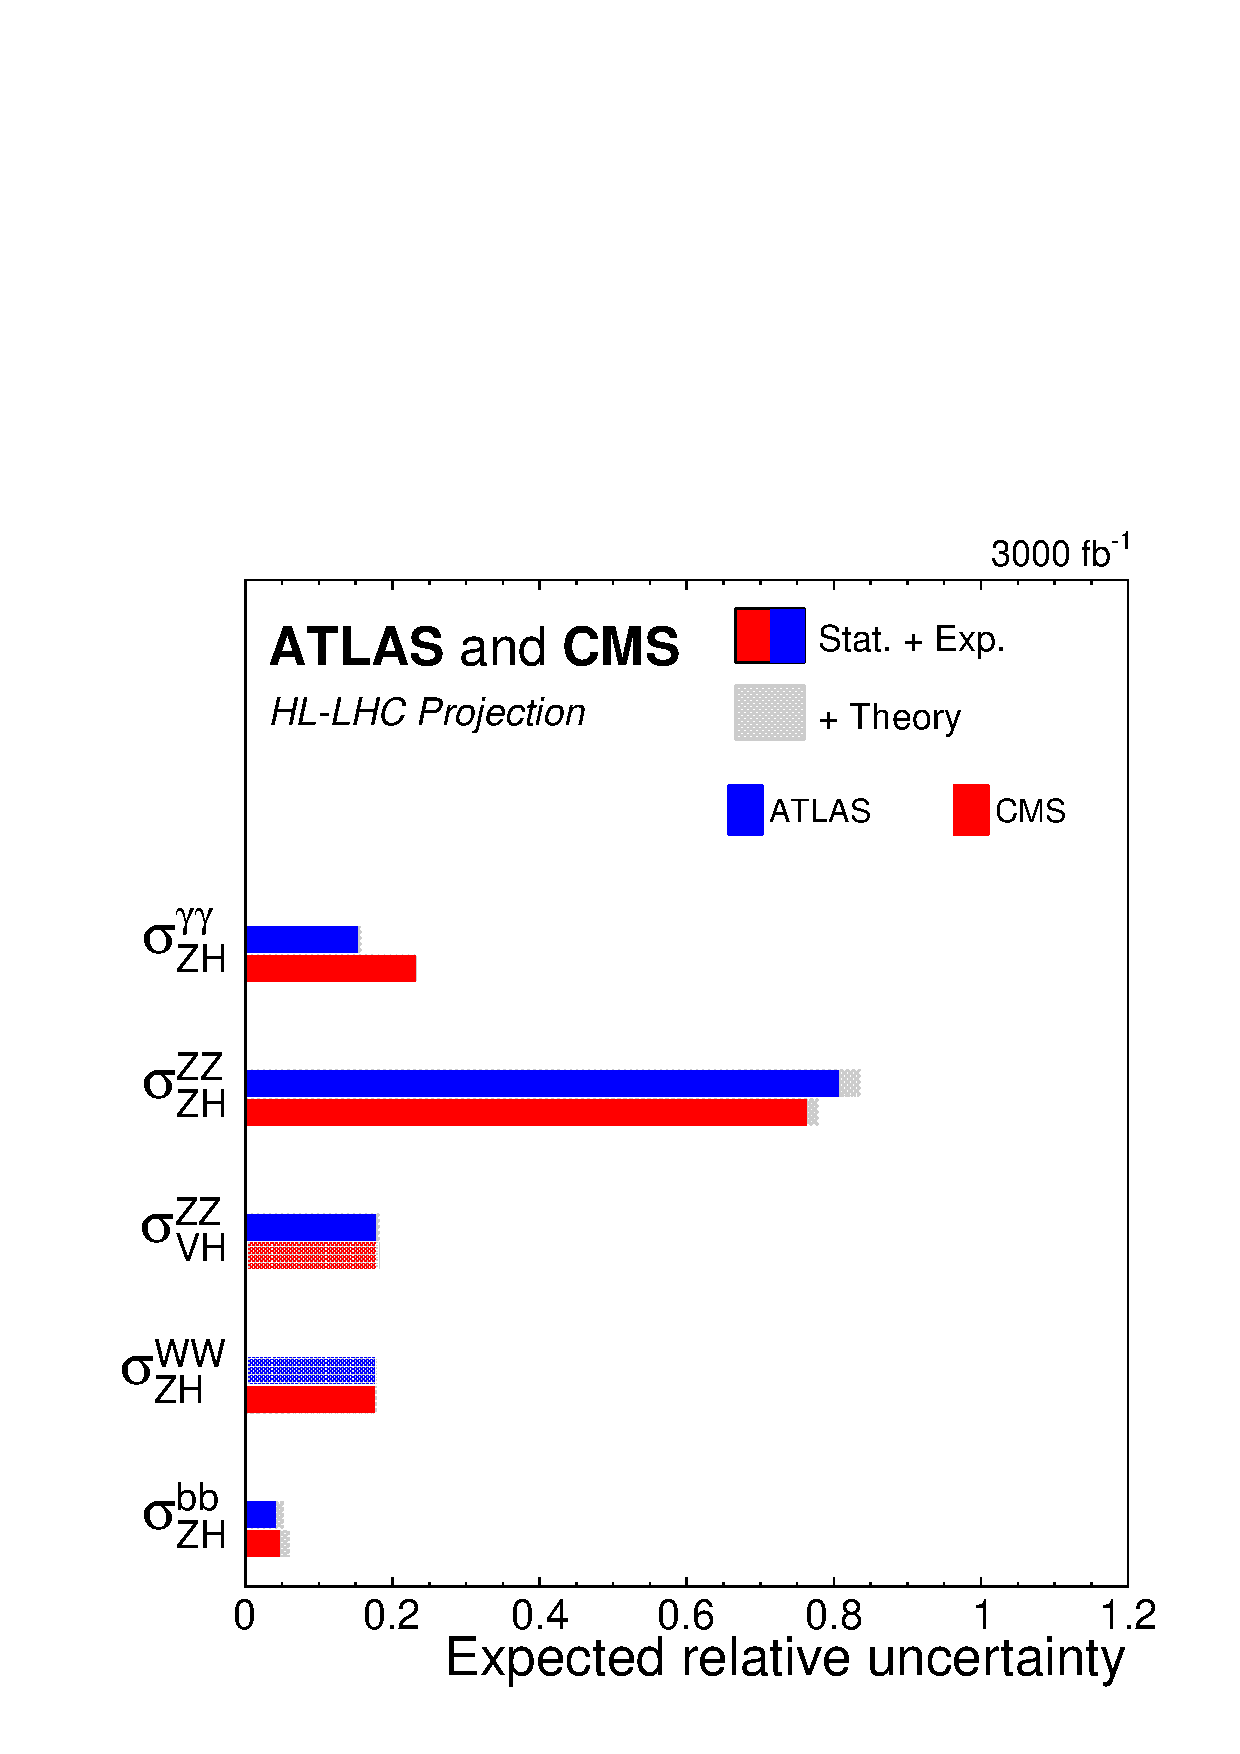
\includegraphics[height=0.332\textheight]{\main/section2/plots/comb/yr_combined_summary_A1_5PD_3000_ZH.pdf}%
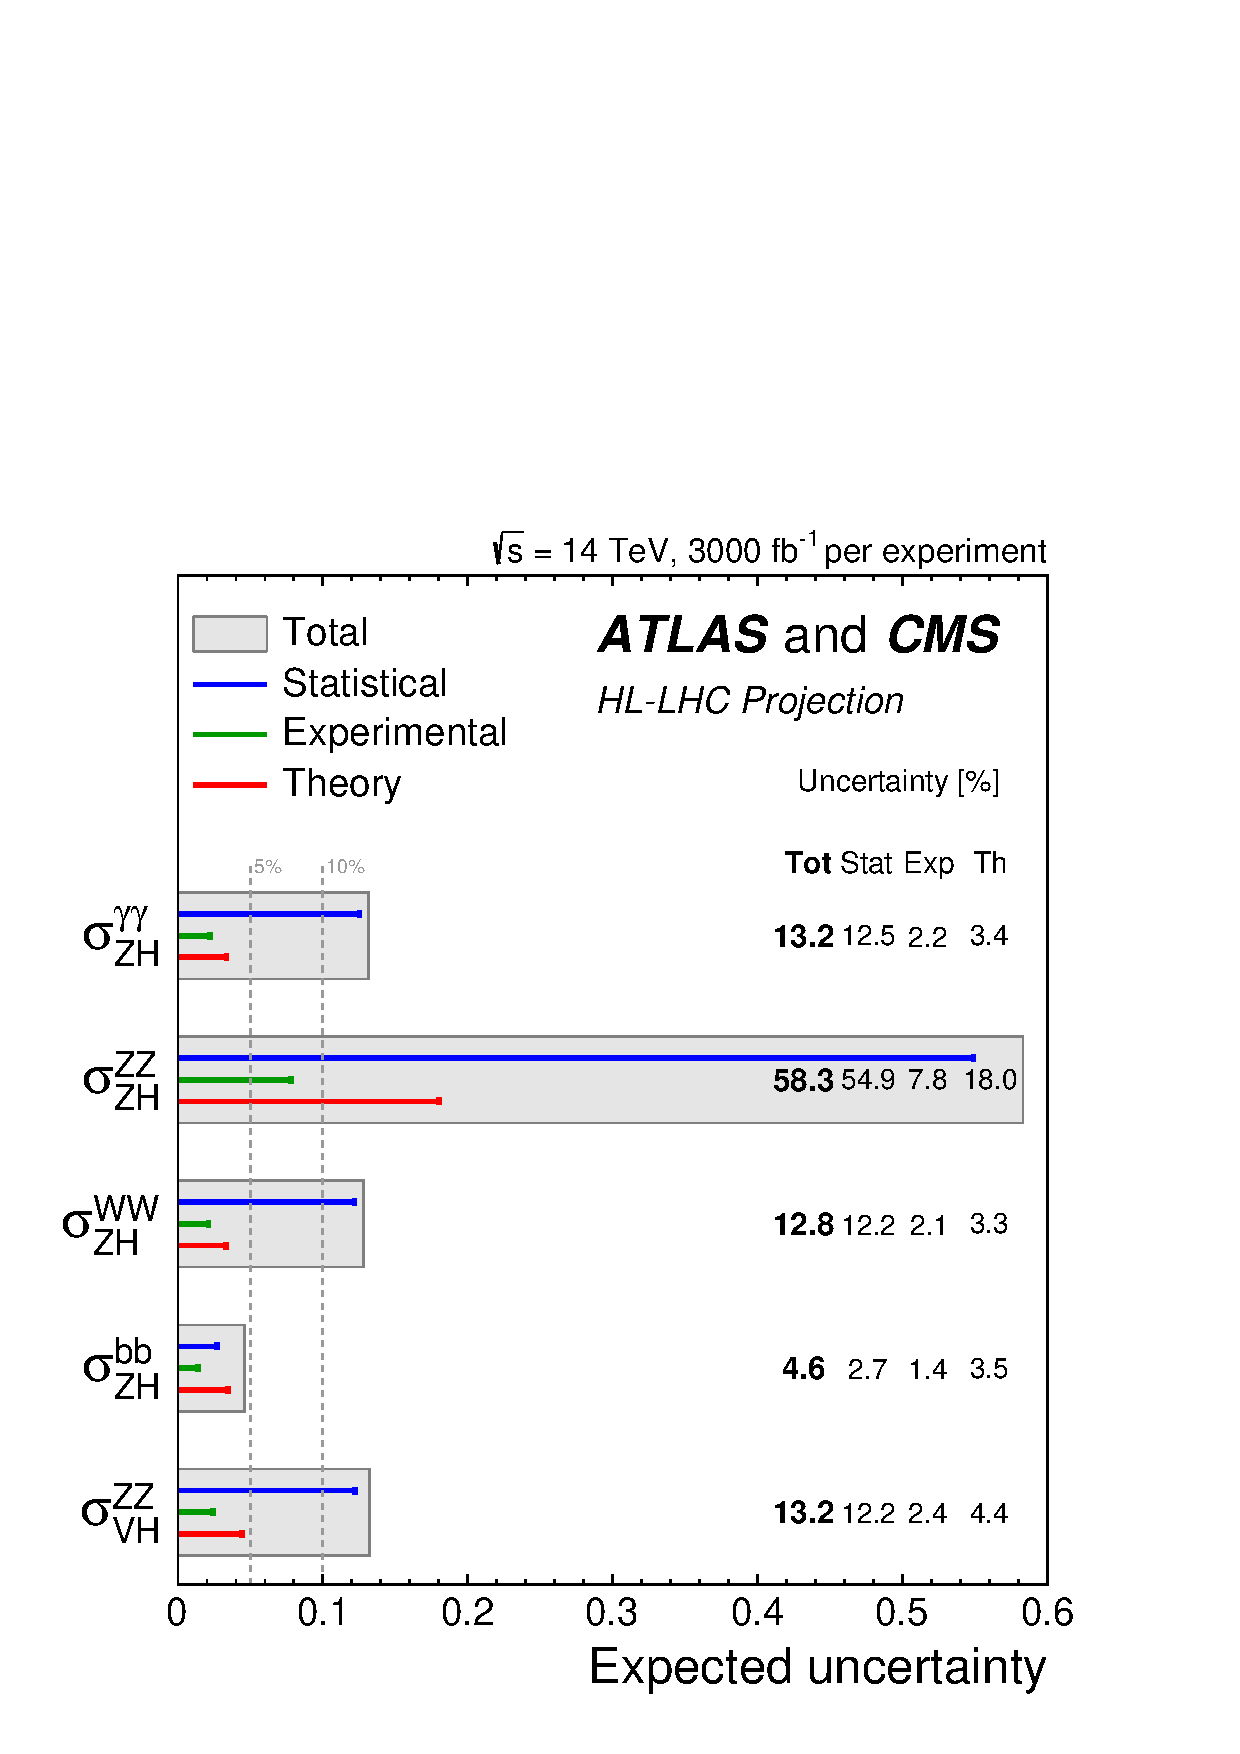
\includegraphics[height=0.33\textheight]{\main/section2/plots/comb/yr_combined_5PD_ZH.pdf}%
\caption{(left) Summary plot showing the total expected $\pm 1\sigma$ uncertainties in S2 (with YR18 systematic uncertainties) on the \wh (top) and \zh (bottom) production cross sections in the different decay modes normalised to the SM predictions   for ATLAS(blue)  and CMS (red). The filled coloured box corresponds to the statistical and experimental systematic uncertainties, while the hatched grey area represent the additional contribution to the total uncertainty due to theoretical systematic uncertainties. In the cases where  the extrapolation is performed only by one experiment, same performances are assumed for the other experiment and this is indicated by a  hatched bar.
(right) Summary plot showing the total expected $\pm 1\sigma$  uncertainties in S2 (with YR18 systematic uncertainties) on the \wh (top) and \zh (bottom) production cross sections in the different decay modes normalised to the SM predictions for the combination of ATLAS and CMS extrapolations. For each measurement,  the total uncertainty is indicated by a grey box while the statistical, experimental and theory uncertainties are indicated by a blue, green and red line respectively. In addition, the numerical values are also reported.}
\label{fig:summary_A1_5PD_WH_ZH}
\end{figure}


\begin{figure}[hbtp]
\centering
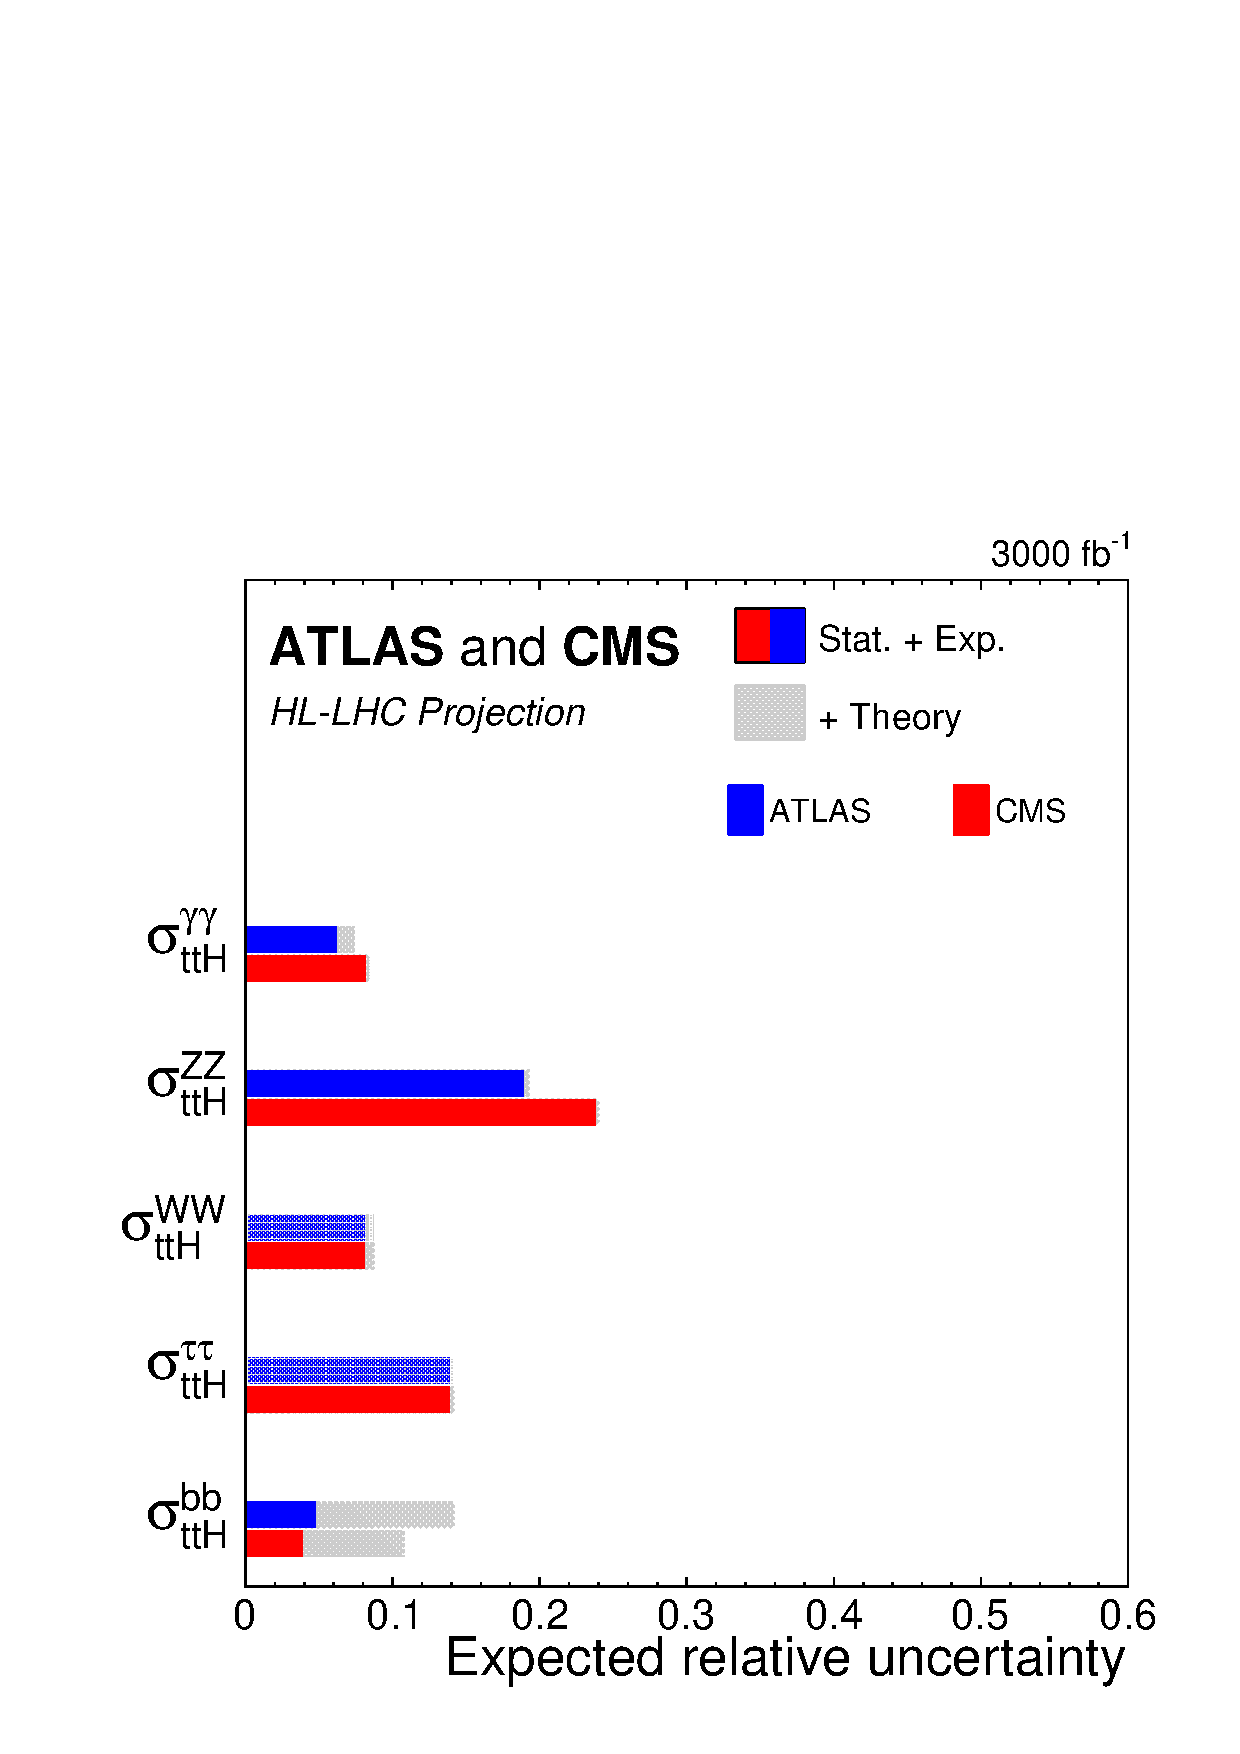
\includegraphics[height=0.332\textheight]{\main/section2/plots/comb/yr_combined_summary_A1_5PD_3000_ttH.pdf}%
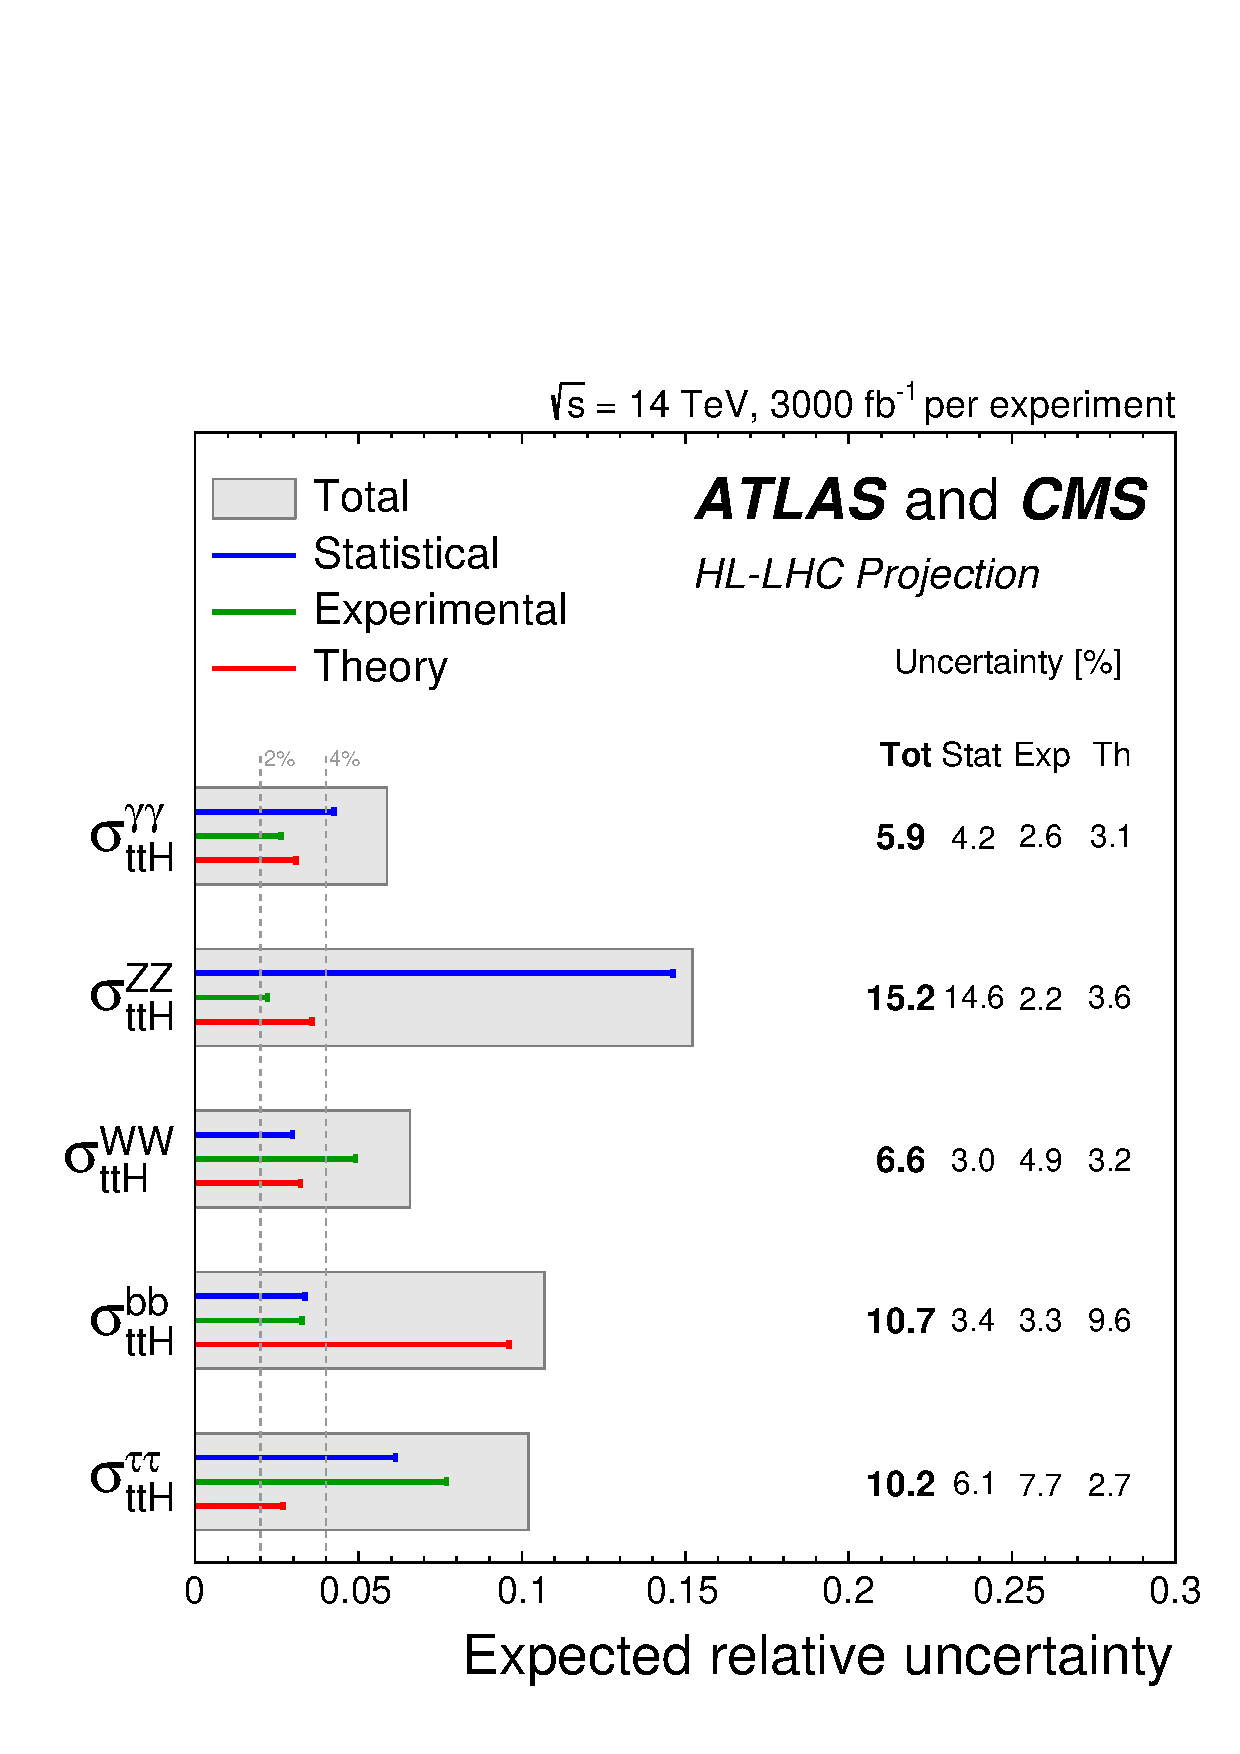
\includegraphics[height=0.33\textheight]{\main/section2/plots/comb/yr_combined_5PD_ttH.pdf}
\caption{(left) Summary plot showing the total expected $\pm 1\sigma$ uncertainties in S2 (with YR18 systematic uncertainties) on the \tth production cross section in the different decay modes normalised to the SM predictions   for ATLAS (blue)  and CMS (red). The filled coloured box corresponds to the statistical and experimental systematic uncertainties, while the hatched grey area represent the additional contribution to the total uncertainty due to theoretical systematic uncertainties. In the cases where  the extrapolation is performed only by one experiment, same performances are assumed for the other experiment and this is indicated by a  hatched bar.
(right) Summary plot showing the total expected $\pm 1\sigma$  uncertainties in S2 (with YR18 systematic uncertainties) on the \tth production cross sections in the different decay modes normalised to the SM predictions for the combination of ATLAS and CMS extrapolations. For each measurement,  the total uncertainty is indicated by a grey box while the statistical, experimental and theory uncertainties are indicated by a blue, green and red line respectively. In addition, the numerical values are also reported.}
\label{fig:summary_A1_5PD_ttH}
\end{figure}


\begin{table}[hbtp]
\centering
\caption{The expected $\pm 1\sigma$ uncertainties, expressed as percentages, on the per-production-mode cross sections in the different decay modes  for ATLAS (left) and CMS (right). Values are given for both S1 (with Run~2 systematic uncertainties~\cite{Sirunyan:2018koj}) and S2 (with YR18 systematic uncertainties). The total uncertainty is decomposed into four components: statistical (Stat), signal theory (SigTh), background theory (BkgTh) and experimental (Exp).}
\scriptsize	
\begin{tabular}{@{} l c c@{\hskip 0.15in} c c c c @{}}
  \hline
   \multicolumn{7}{c}{ATLAS}\\
 \hline
  &  & \multicolumn{5}{c}{3000 $\text{fb}^{-1}$ uncertainty [\%]} \\
  &  & Total & Stat & Exp & SigAcc & BkgTh \\
  \hline
  \multirow{2}{*}{$\sigma_{\mathrm{ggH}}^{\gamma \gamma }$} & S1 &5.2   & 1.7   & 4.7   & 1.1   & 1.2  \\[1pt] 
  & S2 &3.6   & 1.7   & 3.0   & 0.9   & 0.5  \\[4pt] 
  \multirow{2}{*}{$\sigma_{\mathrm{ggH}}^{\mathrm{ZZ}}$} & S1 &4.9   & 2.0   & 3.7   & 1.8   & 1.9  \\[1pt]
  & S2 &3.9   & 2.0   & 3.0   & 1.0   & 1.0  \\[4pt]
  \multirow{2}{*}{$\sigma_{\mathrm{ggH}}^{\mathrm{WW}}$} & S1 &6.0   & 1.2   & 3.2   & 3.7   & 3.4  \\[1pt]
  & S2 &4.3   & 1.2   & 2.7   & 2.1   & 2.4  \\[4pt]
  \multirow{2}{*}{$\sigma_{\mathrm{ggH}}^{\tau \tau }$} & S1 &10.6  & 3.3   & 5.0   & 7.5   & 4.4  \\[1pt]
  & S2 &8.2   & 3.3   & 4.4   & 5.4   & 2.7  \\[4pt]
  \multirow{2}{*}{$\sigma_{\mathrm{ggH}}^{\mu \mu}$} & S1  &19.9  & 17.9  & 2.8   & 8.0   & 0.1  \\[1pt]
  & S2 &18.5  & 17.9  & 2.7   & 3.8   & 0.1  \\[4pt]
  \multirow{2}{*}{$\sigma_{\mathrm{ggH}}^{\mathrm{Z} \gamma }$} & S1 &33.3  & 31.1  & 4.9   & 10.1  & 0.3  \\[1pt]
  & S2 &33.3  & 31.1  & 4.9   & 10.1  & 0.3  \\[4pt]
  \multirow{2}{*}{$\sigma_{\mathrm{VBF}}^{\gamma \gamma }$} & S1  &12.0  & 4.4   & 7.3   & 8.2   & 2.1  \\[1pt]
  & S2 &8.9   & 4.4   & 5.5   & 5.4   & 0.9  \\[4pt]
  \multirow{2}{*}{$\sigma_{\mathrm{VBF}}^{\mathrm{ZZ}}$} & S1 &13.0  & 9.6   & 5.1   & 6.8   & 2.1  \\[1pt]
  & S2 &11.8  & 9.6   & 5.1   & 4.5   & 1.2  \\[4pt]
  \multirow{2}{*}{$\sigma_{\mathrm{VBF}}^{\mathrm{WW}}$} & S1 &10.3  & 3.3   & 3.9   & 7.7   & 4.5  \\[1pt]
  & S2 &6.6   & 3.3   & 2.9   & 4.0   & 2.8  \\[4pt]
  \multirow{2}{*}{$\sigma_{\mathrm{VBF}}^{\tau \tau }$} & S1 &8.7   & 3.7   & 4.1   & 5.5   & 3.8  \\[1pt]
  & S2 &7.8   & 3.7   & 4.8   & 3.2   & 3.6  \\[4pt]
  \multirow{2}{*}{$\sigma_{\mathrm{VBF}}^{\mu \mu }$} & S1 &38.7  & 32.5  & 11.7  & 17.1  & 0.2  \\[1pt]
  & S2 &36.1  & 32.5  & 11.7  & 10.4  & 0.3  \\[4pt]
  \multirow{2}{*}{$\sigma_{\mathrm{VBF}}^{\mathrm{Z} \gamma }$} & S1 &68.2  & 62.2  & 10.9  & 25.0  & 0.5  \\[1pt]
  & S2 &68.2  & 62.2  & 10.9  & 25.0  & 0.5  \\[4pt]
  \multirow{2}{*}{$\sigma_{\mathrm{WH}}^{\gamma \gamma }$} & S1 &14.8  & 13.1  & 5.2   & 4.0   & 1.3  \\[1pt]
  & S2 &13.8  & 13.1  & 3.3   & 2.8   & 0.7  \\[4pt]
  \multirow{2}{*}{$\sigma_{\mathrm{VH}}^{\mathrm{ZZ}}$} & S1 &18.7  & 17.3  & 4.2   & 5.4   & 2.2  \\[1pt]
  & S2 &18.1  & 17.3  & 3.4   & 4.1   & 1.7  \\[4pt]
  \multirow{2}{*}{$\sigma_{\mathrm{WH}}^{\mathrm{bb}}$} & S1 &14.1  & 4.3   & 4.9   & 7.3   & 10.1 \\[1pt]
  & S2 &10.1  & 4.4   & 4.1   & 4.2   & 6.9  \\[4pt]
  \multirow{2}{*}{$\sigma_{\mathrm{ZH}}^{\gamma \gamma }$} & S1 &17.0  & 14.9  & 5.1   & 6.3   & 1.3  \\[1pt]
  & S2 &15.7  & 14.9  & 3.2   & 3.7   & 0.6  \\[4pt]
  \multirow{2}{*}{$\sigma_{\mathrm{ZH}}^{\mathrm{bb}}$} & S1 &7.0   & 3.5   & 2.7   & 4.0   & 3.6  \\[1pt]
  & S2 &5.2   & 3.5   & 2.0   & 2.1   & 2.4  \\[4pt]
  \multirow{2}{*}{$\sigma_{\mathrm{ttH}}^{\gamma \gamma }$} & S1 &10.0  & 4.6   & 5.9   & 6.4   & 1.5  \\[1pt]
  & S2 &7.4   & 4.6   & 4.1   & 3.9   & 0.5  \\[4pt]
  \multirow{2}{*}{$\sigma_{\mathrm{ttH}}^{\mathrm{ZZ}}$} & S1 &20.5  & 18.6  & 4.1   & 7.3   & 1.7  \\[1pt]
  & S2 &19.3  & 18.6  & 3.1   & 3.8   & 0.9  \\[4pt]
  \multirow{2}{*}{$\sigma_{\mathrm{ttH}}^{\mathrm{WW} \tau \tau}$} & S1 &22.1  & 6.3   & 18.2  & 7.0   & 8.1  \\[1pt]
  & S2 &20.2  & 6.3   & 17.9  & 4.3   & 5.1  \\[4pt]
  \multirow{2}{*}{$\sigma_{\mathrm{ttH}}^{\mathrm{bb}}$} & S1 &19.9  & 3.2   & 4.2   & 7.4   & 17.8 \\[1pt]
  & S2 &14.2  & 3.2   & 3.4   & 4.4   & 12.7 \\[4pt]
  \hline
\end{tabular}
\hspace{0.5cm}
\begin{tabular}{@{} l c c@{\hskip 0.15in} c c c c @{}}
 \hline
  &  & \multicolumn{5}{c}{3000 $\text{fb}^{-1}$ uncertainty [\%]} \\
  &  & Total & Stat & Exp & SigAcc & BkgTh \\
 \hline
\multirow{2}{*}{$\sigma_{\mathrm{ggH}}^{\gamma \gamma }$} & S1  & 3.9& 1.9 & 3.3 & 0.7 & 1.0  \\[1pt]
                        & S2  & 2.8& 1.9 & 2.1 & 0.8 & 0.9  \\[4pt]
\multirow{2}{*}{$\sigma_{\mathrm{ggH}}^{\mathrm{ZZ}}$} & S1  & 4.1& 2.1 & 2.7 & 1.2 & 1.7  \\[1pt]
                        & S2  & 3.0& 2.1 & 1.8 & 0.8 & 0.7  \\[4pt]
\multirow{2}{*}{$\sigma_{\mathrm{ggH}}^{\mathrm{WW}}$} & S1  & 3.6& 1.2 & 1.5 & 2.9 & 1.0  \\[1pt]
                        & S2  & 2.5& 1.2 & 1.2 & 1.6 & 0.9  \\[4pt]
\multirow{2}{*}{$\sigma_{\mathrm{ggH}}^{\tau \tau }$} & S1  & 5.7& 2.6 & 3.5 & 3.3 & 1.7  \\[1pt]
                        & S2  & 4.6& 2.6 & 2.9 & 2.3 & 0.7  \\[4pt]
\multirow{2}{*}{$\sigma_{\mathrm{ggH}}^{\mathrm{bb}}$} & S1  & 34.3& 20.6 & 10.0 & 23.7 & 3.2  \\[1pt]
                        & S2  & 24.7& 20.6 & 2.6 & 12.2 & 1.5  \\[4pt]
\multirow{2}{*}{$\sigma_{\mathrm{ggH}}^{\sigma \sigma }$} & S1  & 15.9& 13.4 & 8.0 & 2.6 & 1.9  \\[1pt]
                        & S2  & 13.5& 13.4 & 2.0 & 1.4 & 0.6  \\[4pt]
\multirow{2}{*}{$\sigma_{\mathrm{VBF}}^{\gamma \gamma }$} & S1  & 22.1& 5.2 & 19.9 & 7.9 & 1.3  \\[1pt]
                        & S2  & 12.7& 5.2 & 10.9 & 4.0 & 0.3  \\[4pt]
\multirow{2}{*}{$\sigma_{\mathrm{VBF}}^{\mathrm{ZZ}}$} & S1  & 15.1& 11.7 & 1.8 & 8.8 & 2.4  \\[1pt]
                        & S2  & 13.3& 11.7 & 1.3 & 5.9 & 0.8  \\[4pt]
\multirow{2}{*}{$\sigma_{\mathrm{VBF}}^{\mathrm{WW}}$} & S1  & 8.1& 6.3 & 2.0 & 4.4 & 1.8  \\[1pt]
                        & S2  & 7.2& 6.3 & 1.6 & 2.8 & 1.1  \\[4pt]
\multirow{2}{*}{$\sigma_{\mathrm{VBF}}^{\tau \tau }$} & S1  & 4.9& 3.8 & 2.0 & 2.8 & 1.5  \\[1pt]
                        & S2  & 4.2& 3.8 & 1.3 & 1.2 & 0.4  \\[4pt]
\multirow{2}{*}{$\sigma_{\mathrm{VBF}}^{\sigma \sigma }$} & S1  & 57.3& 53.2 & 11.3 & 18.0 & 4.5  \\[1pt]
                        & S2  & 54.0& 53.2 & 2.6 & 9.5 & 1.0  \\[4pt]
\multirow{2}{*}{$\sigma_{\mathrm{WH}}^{\gamma \gamma }$} & S1  & 14.3& 13.6 & 3.7 & 2.0 & 1.4  \\[1pt]
                        & S2  & 13.8& 13.6 & 1.7 & 1.5 & 0.2  \\[4pt]
\multirow{2}{*}{$\sigma_{\mathrm{WH}}^{\mathrm{ZZ}}$} & S1  & 47.9& 46.5 & 7.8 & 11.2 & 2.8  \\[1pt]
                        & S2  & 47.8& 46.5 & 3.8 & 4.0 & 0.8  \\[4pt]
\multirow{2}{*}{$\sigma_{\mathrm{WH}}^{\mathrm{WW}}$} & S1  & 15.6& 12.9 & 6.5 & 5.3 & 2.2  \\[1pt]
                        & S2  & 13.7& 12.9 & 3.1 & 2.9 & 1.5  \\[4pt]
\multirow{2}{*}{$\sigma_{\mathrm{WH}}^{\mathrm{bb}}$} & S1  & 16.0& 5.6 & 9.8 & 5.3 & 10.8  \\[1pt]
                        & S2  & 9.4& 5.6 & 5.1 & 2.2 & 5.1  \\[4pt]
\multirow{2}{*}{$\sigma_{\mathrm{ZH}}^{\gamma \gamma }$} & S1  & 23.5& 23.1 & 2.9 & 3.1 & 1.5  \\[1pt]
                        & S2  & 23.2& 23.1 & 1.2 & 2.4 & 0.4  \\[4pt]
\multirow{2}{*}{$\sigma_{\mathrm{ZH}}^{\mathrm{ZZ}}$} & S1  & 82.3& 75.7 & 16.4 & 26.3 & 7.6  \\[1pt]
                        & S2  & 78.4& 75.7 & 9.9 & 15.1 & 1.3  \\[4pt]
\multirow{2}{*}{$\sigma_{\mathrm{ZH}}^{\mathrm{WW}}$} & S1  & 18.5& 17.2 & 3.5 & 5.3 & 2.4  \\[1pt]
                        & S2  & 17.7& 17.2 & 3.0 & 2.8 & 1.7  \\[4pt]
\multirow{2}{*}{$\sigma_{\mathrm{ZH}}^{\mathrm{bb}}$} & S1  & 7.9& 4.2 & 2.3 & 5.6 & 3.1  \\[1pt]
                        & S2  & 6.0& 4.2 & 1.9 & 2.9 & 2.6  \\[4pt]
\multirow{2}{*}{$\sigma_{\mathrm{ttH}}^{\gamma \gamma }$} & S1  & 9.3& 7.7 & 3.9 & 3.5 & 1.0  \\[1pt]
                        & S2  & 8.4& 7.7 & 2.7 & 1.9 & 0.2  \\[4pt]
\multirow{2}{*}{$\sigma_{\mathrm{ttH}}^{\mathrm{ZZ}}$} & S1  & 24.6& 23.6 & 4.2 & 4.9 & 2.5  \\[1pt]
                        & S2  & 24.2& 23.6 & 3.1 & 2.6 & 1.8  \\[4pt]
\multirow{2}{*}{$\sigma_{\mathrm{ttH}}^{\mathrm{WW}}$} & S1  & 11.2& 4.2 & 9.1 & 1.8 & 4.5  \\[1pt]
                        & S2  & 8.7& 4.2 & 6.9 & 1.1 & 3.0  \\[4pt]
\multirow{2}{*}{$\sigma_{\mathrm{ttH}}^{\mathrm{bb}}$} & S1  & 15.9& 2.8 & 3.9 & 0.0 & 15.2  \\[1pt]
                        & S2  & 10.8& 2.8 & 2.7 & 0.1 & 10.0  \\[4pt]
\multirow{2}{*}{$\sigma_{\mathrm{ttH}}^{\tau \tau }$} & S1  & 16.5& 8.7 & 13.1 & 3.4 & 3.5  \\[1pt]
                        & S2  & 14.2& 8.7 & 10.9 & 1.6 & 2.1  \\[4pt]
\hline
\end{tabular}
\label{tab:summary_A1_5PD}
\vspace{0.5cm}
\end{table}


%Figure~\ref{fig:comb_5PD} shows the expected $\pm 1\sigma$ uncertainties for the combined ATLAS-CMS projections of the Higgs boson production mode cross-sections in different decay channels normalized to the corresponding SM values for S2.

%\begin{figure}[hbtp]
%\centering
%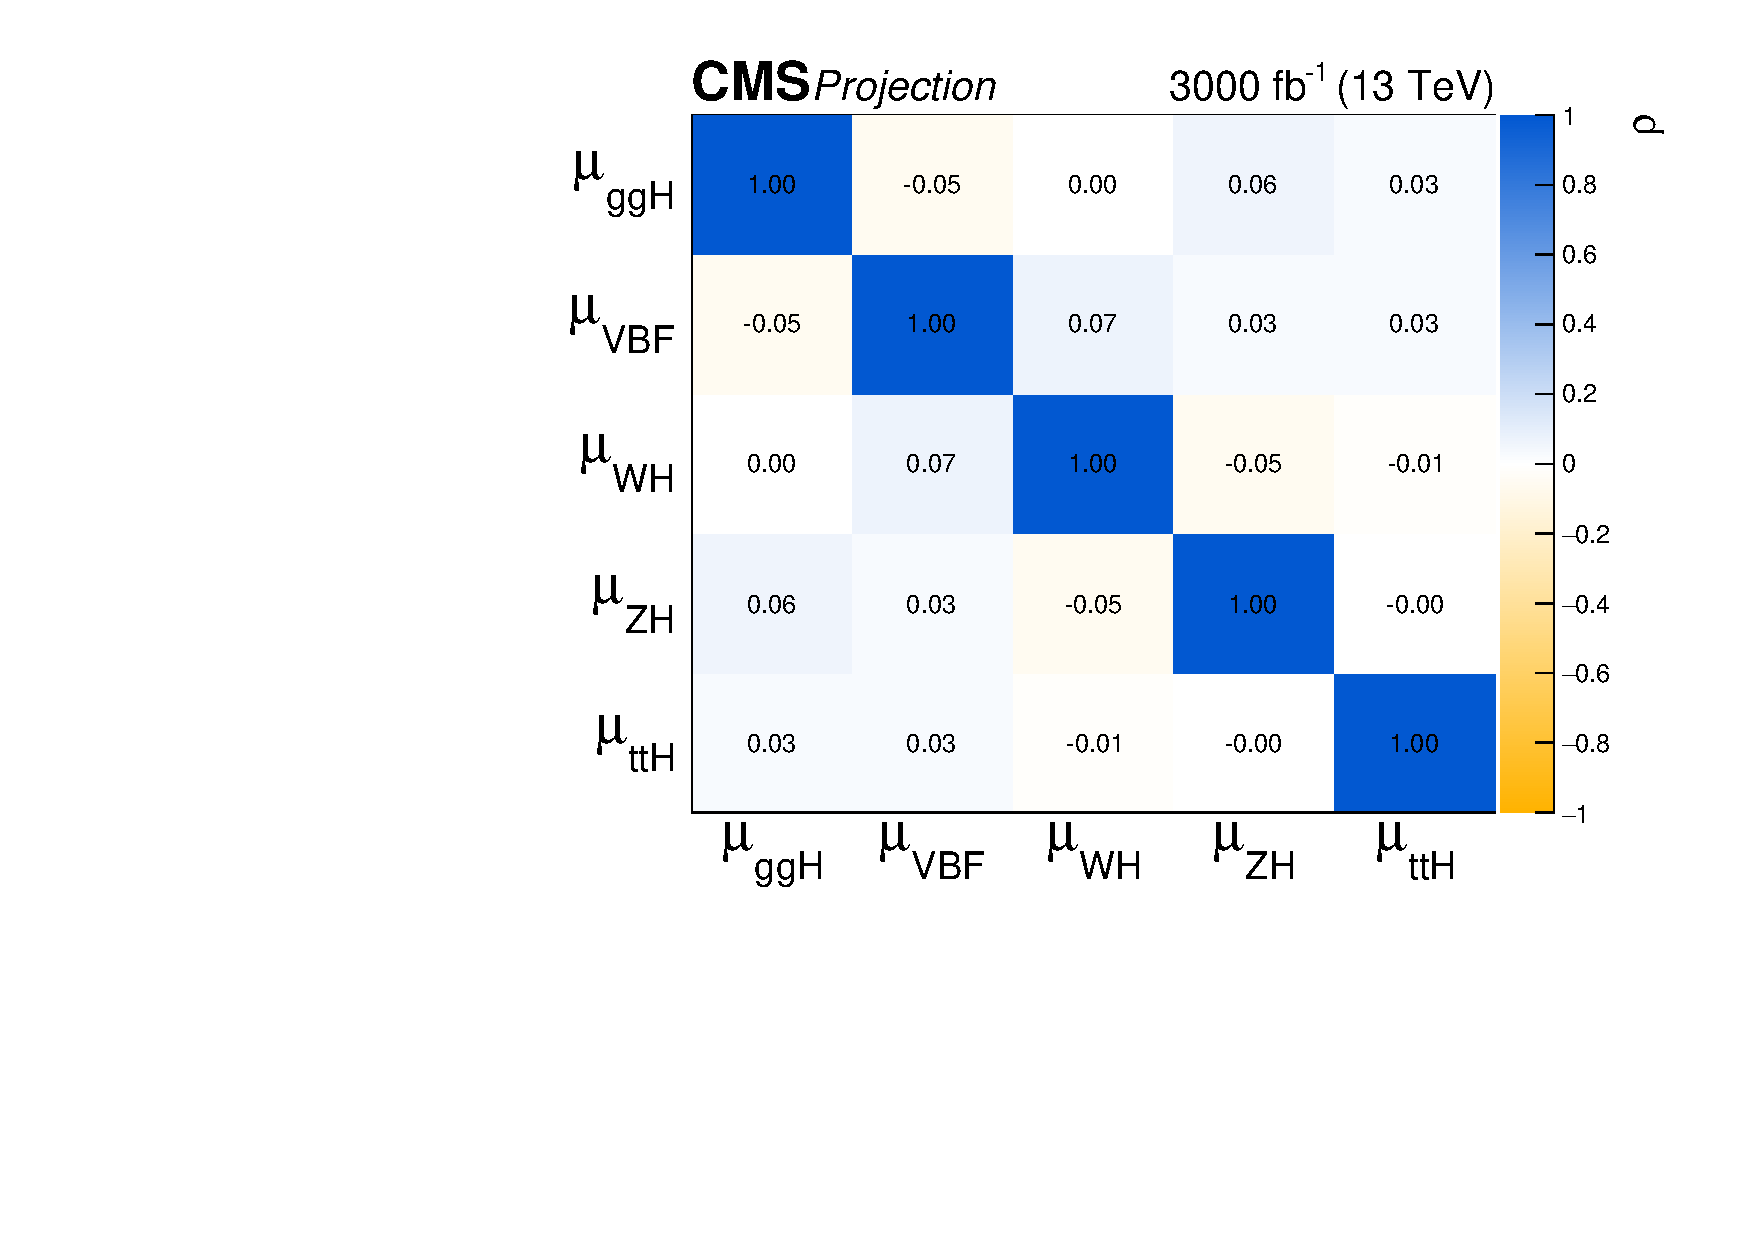
\includegraphics[width=0.48\textwidth]{\main/section2/plots/comb/correlations_A1_5P_S2_3000.pdf}%
%\caption{Summary plot showing the total expected $\pm 1\sigma$ uncertainties in S2  (with YR18 systematic uncertainties) on the Higgs boson production mode cross-sections in different decay channels normalized to the SM predictions combining  ATLAS and CMS.}
%\label{fig:comb_5PD}
%\end{figure}



%-------------------------------------------------------------






%\subsubsection{Signal strength per-production mode}
\subsubsection{Cross sections per-production mode}
%\wip{plots and results to be updated}

The expected $\pm 1\sigma$ relative uncertainties on the per-production-mode cross sections parameters in S2 for ATLAS, CMS and their combination are summarised in Figure~\ref{fig:summary_A1_5P}.
Additionally, the numerical values for the ATLAS-CMS combination  are also given, with the uncertainty decomposed in three components: statistical, experimental and theory.
In scenario S2 the contribution from the statistical, experimental and theoretical uncertainties to the total error for the combined  \ggh and \vbf cross section measurements is similar. For \wh and \zh production cross section measurements, the statistical  and theoretical uncertainty are the dominant one.
Finally, the total uncertainty on the \tth production cross section measurement is dominated by the theoretical uncertainty, which is almost a factor two larger with respect to the other components.
%with numerical values given in Table~\ref{tab:summary_A1_5P}.
%In S1 the signal theory is the main contribution for all modes except $\wh$ which remains limited by statistics. In S2 $\mu_{\vbf}$ and $\mu_{\wh}$ are also statistically limited.
The numerical values of the expected $\pm 1\sigma$ uncertainties on the per-production-mode cross sections for the ATLAS and CMS projections are given in Table~\ref{tab:summary_A1_5P}. The table  gives the breakdown of the uncertainty into four components: statistical, signal theory, background theory and experimental for both scenarios S1 and S2. 

\begin{figure}[hbtp]
\centering
% \includegraphics[width=0.48\textwidth]{\main/section2/plots/comb/summary_A1_5P_300.pdf}%
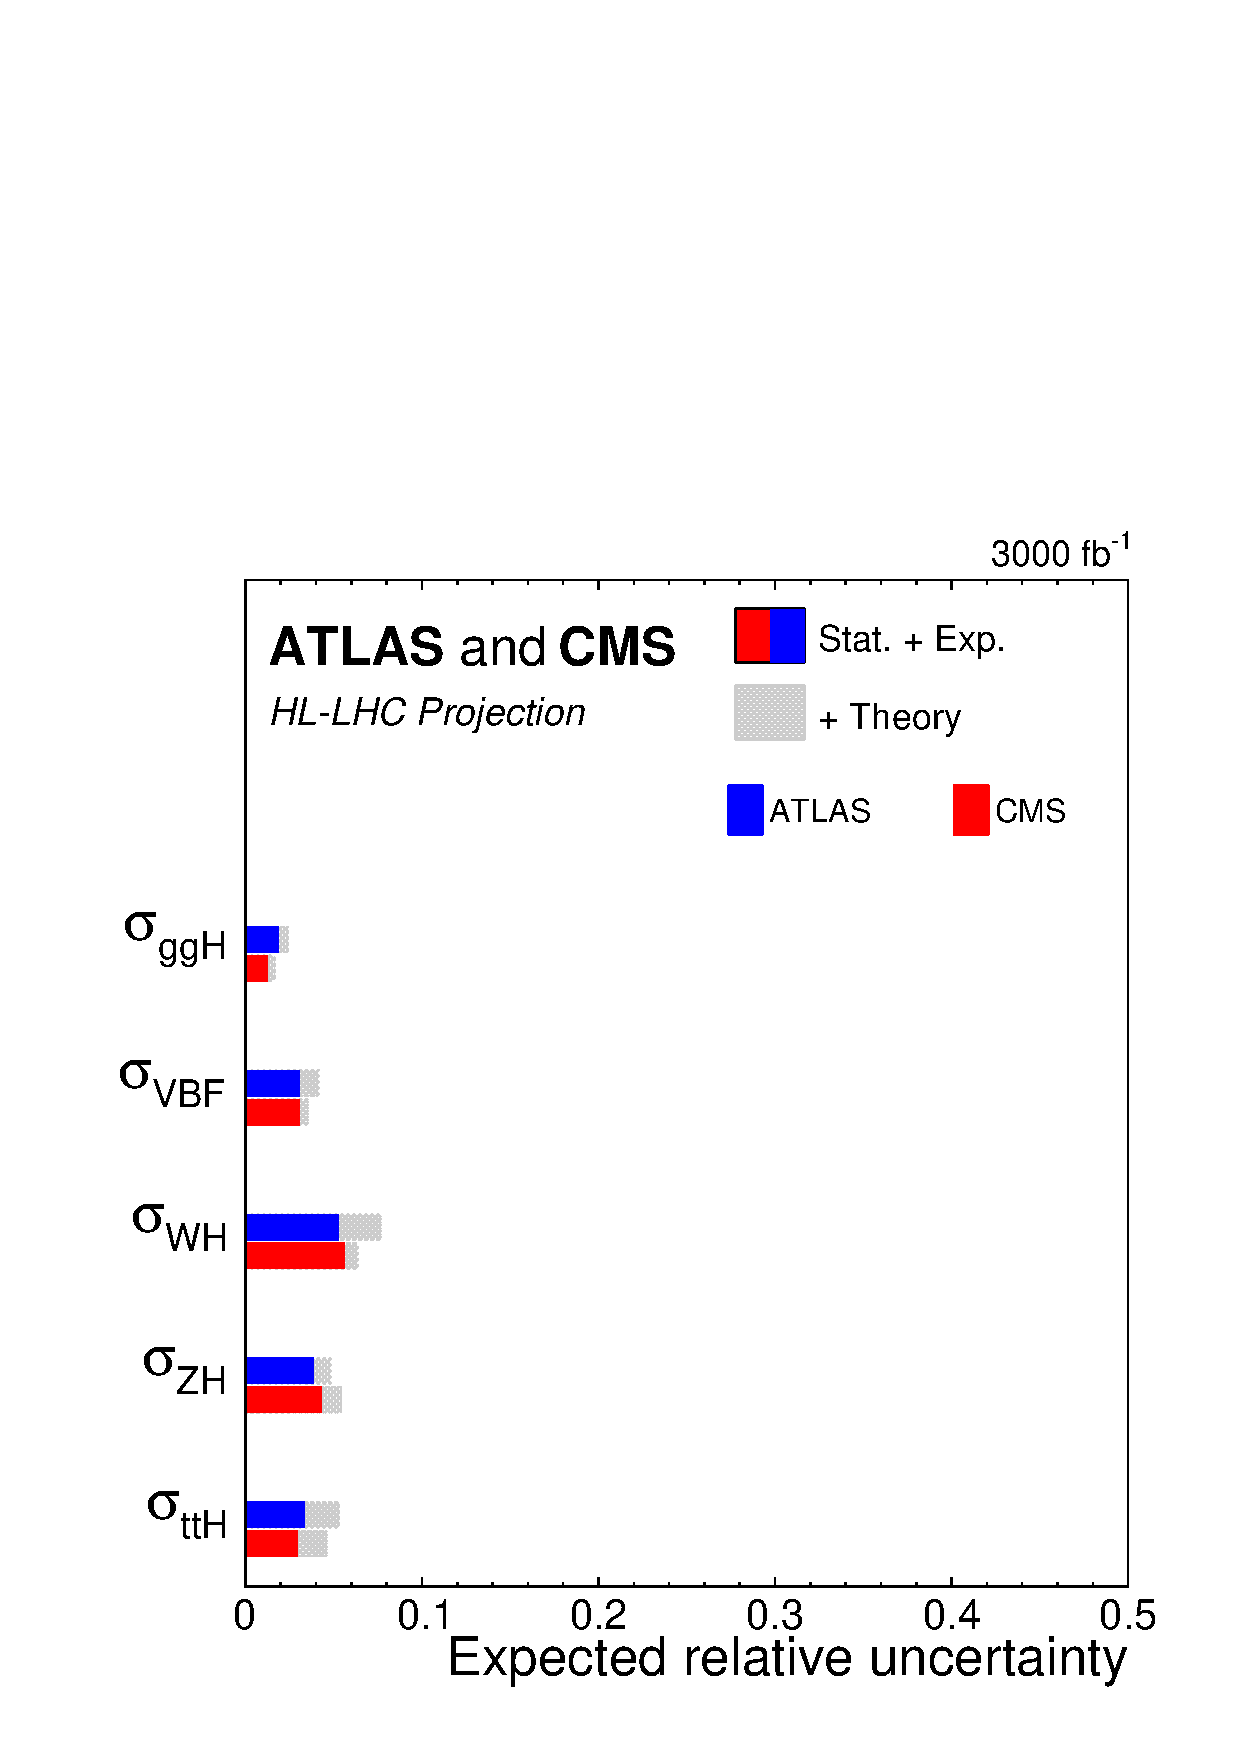
\includegraphics[height=0.332\textheight]{\main/section2/plots/comb/yr_combined_summary_A1_5P_3000.pdf}%
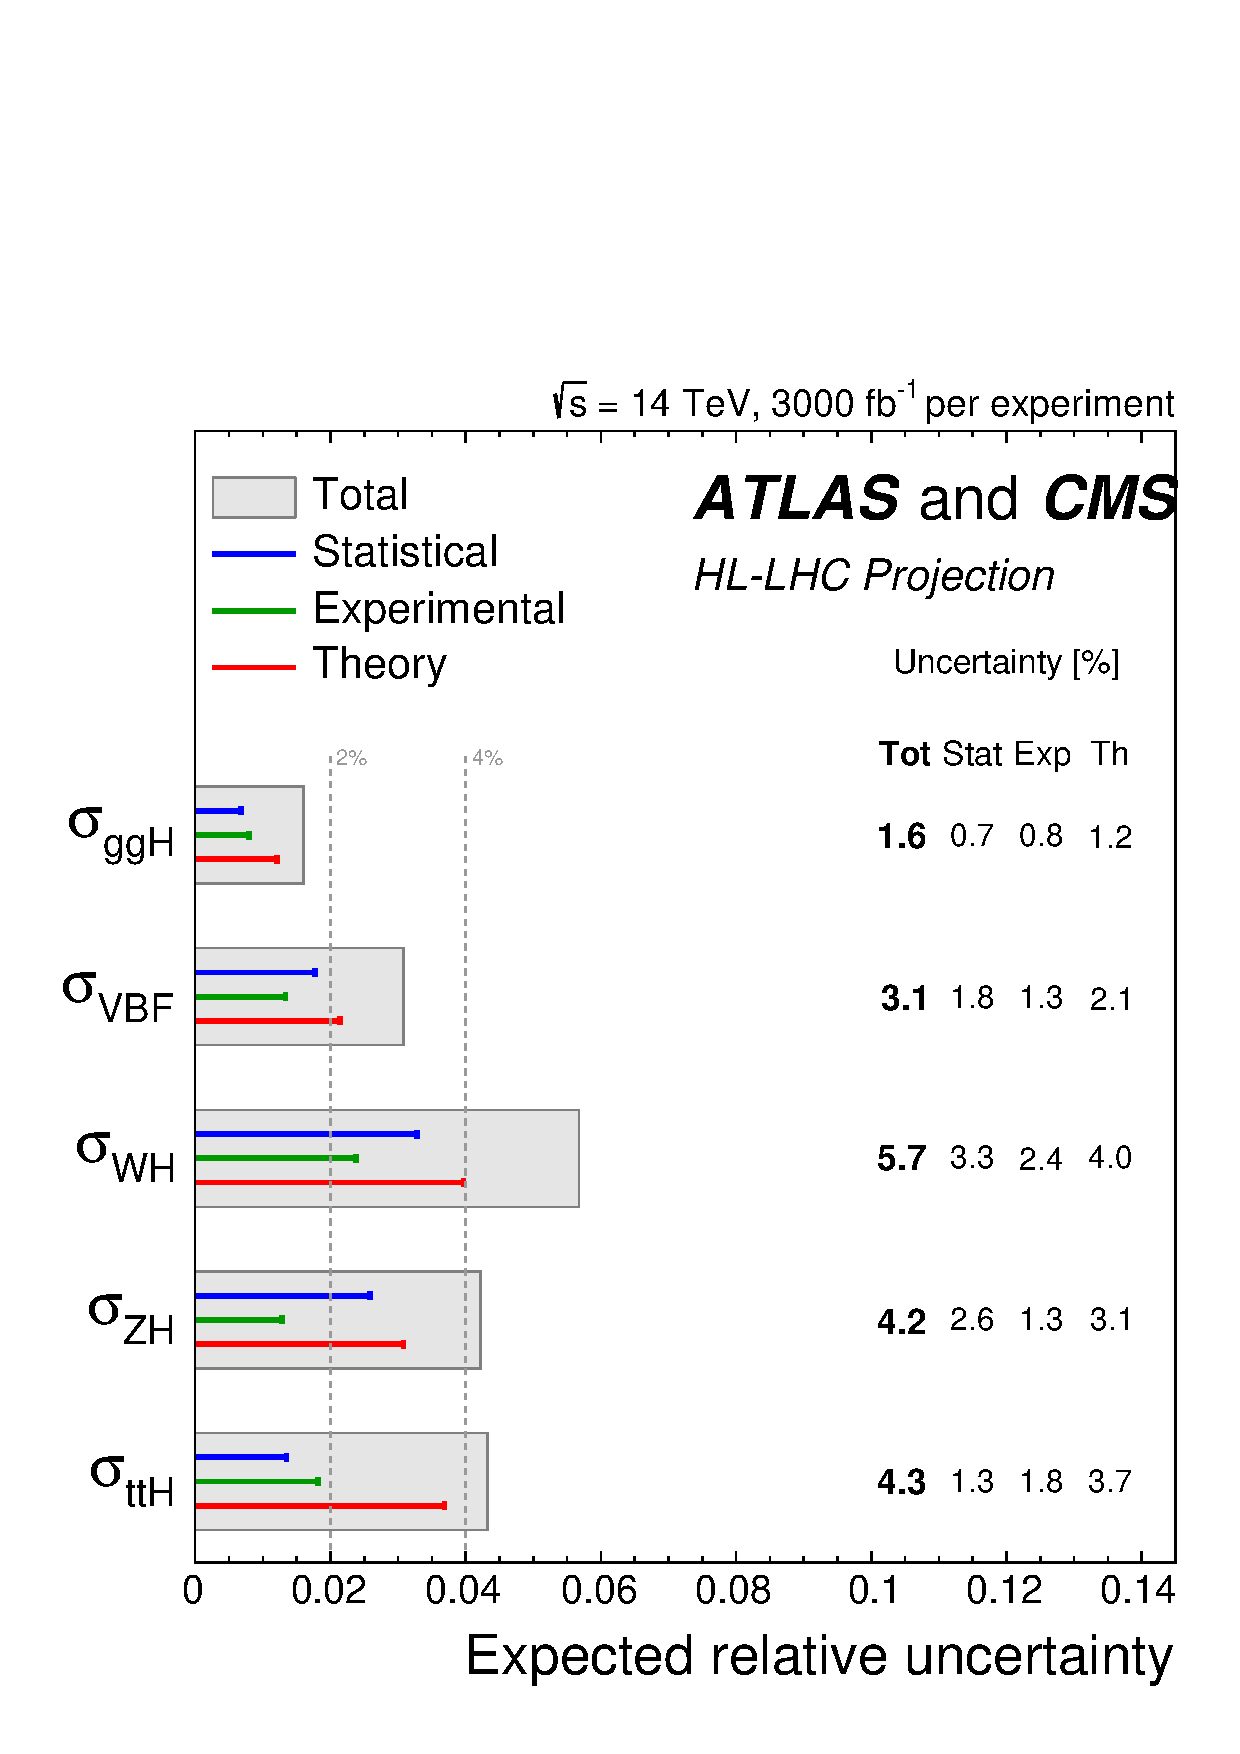
\includegraphics[height=0.33\textheight]{\main/section2/plots/comb/yr_combined_5P.pdf}%
\caption{(left) Summary plot showing the total expected $\pm 1\sigma$ uncertainties in S2 (with YR18 systematic uncertainties) on the  per-production-mode cross sections normalised to the SM predictions   for ATLAS (blue)  and CMS (red). The filled coloured box corresponds to the statistical and experimental systematic uncertainties, while the hatched grey area represent the additional contribution to the total uncertainty due to theoretical systematic uncertainties.
(right) Summary plot showing the total expected $\pm 1\sigma$  uncertainties in S2 (with YR18 systematic uncertainties) on the per-production-mode cross sections normalised to the SM predictions for the combination of ATLAS and CMS extrapolations. For each measurement,  the total uncertainty is indicated by a grey box while the statistical, experimental and theory uncertainties are indicated by a blue, green and red line respectively.  In addition, the numerical values are also reported.}
\label{fig:summary_A1_5P}
\end{figure}


\begin{table}[hbtp]
\centering
\caption{The expected $\pm 1\sigma$ uncertainties, expressed as percentages, on the per-production-mode cross sections normalised to the SM values  for  ATLAS (left) and CMS (right). Values are given for both S1 (with Run~2 systematic uncertainties~\cite{Sirunyan:2018koj}) and S2 (with YR18 systematic uncertainties). The total uncertainty is decomposed into four components: statistical (Stat), signal theory (SigTh), background theory (BkgTh) and experimental (Exp).}
\small
\begin{tabular}{@{} l c c@{\hskip 0.15in} c c c c @{}}
  \hline
   \multicolumn{7}{c}{ATLAS}\\
 \hline  
  &  & \multicolumn{5}{c}{3000 $\text{fb}^{-1}$ uncertainty [\%]} \\
  &  & Total & Stat & Exp & SigTh & BkgTh \\
  \hline
  \multirow{2}{*}{$\sigma_{\mathrm{ggH}}$} & S1 &3.5   & 0.8   & 2.1   & 2.1   & 1.6  \\[1pt]
  & S2 &2.4   & 0.8   & 1.7   & 1.2   & 1.0  \\[4pt]
  \multirow{2}{*}{$\sigma_{\mathrm{VBF}}$} & S1 &5.5   & 2.0   & 2.7   & 3.7   & 2.1  \\[1pt]
  & S2 &4.2   & 2.0   & 2.3   & 2.2   & 1.7  \\[4pt]
  \multirow{2}{*}{$\sigma_{\mathrm{WH}}$} & S1 &9.3   & 4.0   & 4.0   & 5.1   & 5.4  \\[1pt]
  & S2 &7.7   & 4.0   & 3.4   & 3.3   & 4.5  \\[4pt]
  \multirow{2}{*}{$\sigma_{\mathrm{ZH}}$} & S1 &6.2   & 3.4   & 2.4   & 3.4   & 3.0  \\[1pt]
  & S2 &4.8   & 3.4   & 1.8   & 2.0   & 2.1  \\[4pt]
  \multirow{2}{*}{$\sigma_{\mathrm{ttH}}$} & S1 &6.7   & 1.9   & 3.1   & 3.7   & 4.3  \\[1pt]
  & S2 &5.3   & 1.9   & 2.8   & 2.4   & 3.3  \\[4pt]
  \hline
\end{tabular}
\hspace{0.5cm}
\begin{tabular}{@{} l c c@{\hskip 0.15in} c c c c @{}}
 \hline
  &  & \multicolumn{5}{c}{3000 $\text{fb}^{-1}$ uncertainty [\%]} \\
  &  & Total & Stat & Exp & SigTh & BkgTh \\
 \hline
\multirow{2}{*}{$\sigma_{\mathrm{ggH}}$} & S1  & 2.4& 0.8 & 1.2 & 1.6 & 0.9  \\[1pt]
                        & S2  & 1.7& 0.8 & 0.9 & 0.9 & 0.6  \\[4pt]
\multirow{2}{*}{$\sigma_{\mathrm{VBF}}$} & S1  & 4.1& 2.6 & 2.1 & 2.0 & 1.3  \\[1pt]
                        & S2  & 3.5& 2.6 & 1.6 & 1.8 & 0.3  \\[4pt]
\multirow{2}{*}{$\sigma_{\mathrm{WH}}$} & S1  & 8.1& 4.6 & 5.2 & 2.6 & 3.3  \\[1pt]
                        & S2  & 6.4& 4.6 & 3.2 & 1.5 & 2.7  \\[4pt]
\multirow{2}{*}{$\sigma_{\mathrm{ZH}}$} & S1  & 6.7& 3.9 & 2.1 & 4.3 & 2.5  \\[1pt]
                        & S2  & 5.4& 3.9 & 1.7 & 2.4 & 2.3  \\[4pt]
\multirow{2}{*}{$\sigma_{\mathrm{ttH}}$} & S1  & 5.8& 1.8 & 3.1 & 1.9 & 4.1  \\[1pt]
                        & S2  & 4.6& 1.8 & 2.4 & 1.1 & 3.4  \\[4pt]
\hline
\end{tabular}
\label{tab:summary_A1_5P}
\vspace{0.5cm}
\end{table}

%% TO DECIDE IF WE WANT ALSO THE CORR MATRICES


%Figure~\ref{fig:corr_A1_5P} shows the correlation coefficients between the production cross sections  parameters in S2. The correlations in this case are small compared to the per-decay measurements since production modes are generally well-isolated by independent analysis categories and the main theoretical uncertainties on the SM signal expectation are uncorrelated.

%\begin{figure}[hbtp]
%\centering
%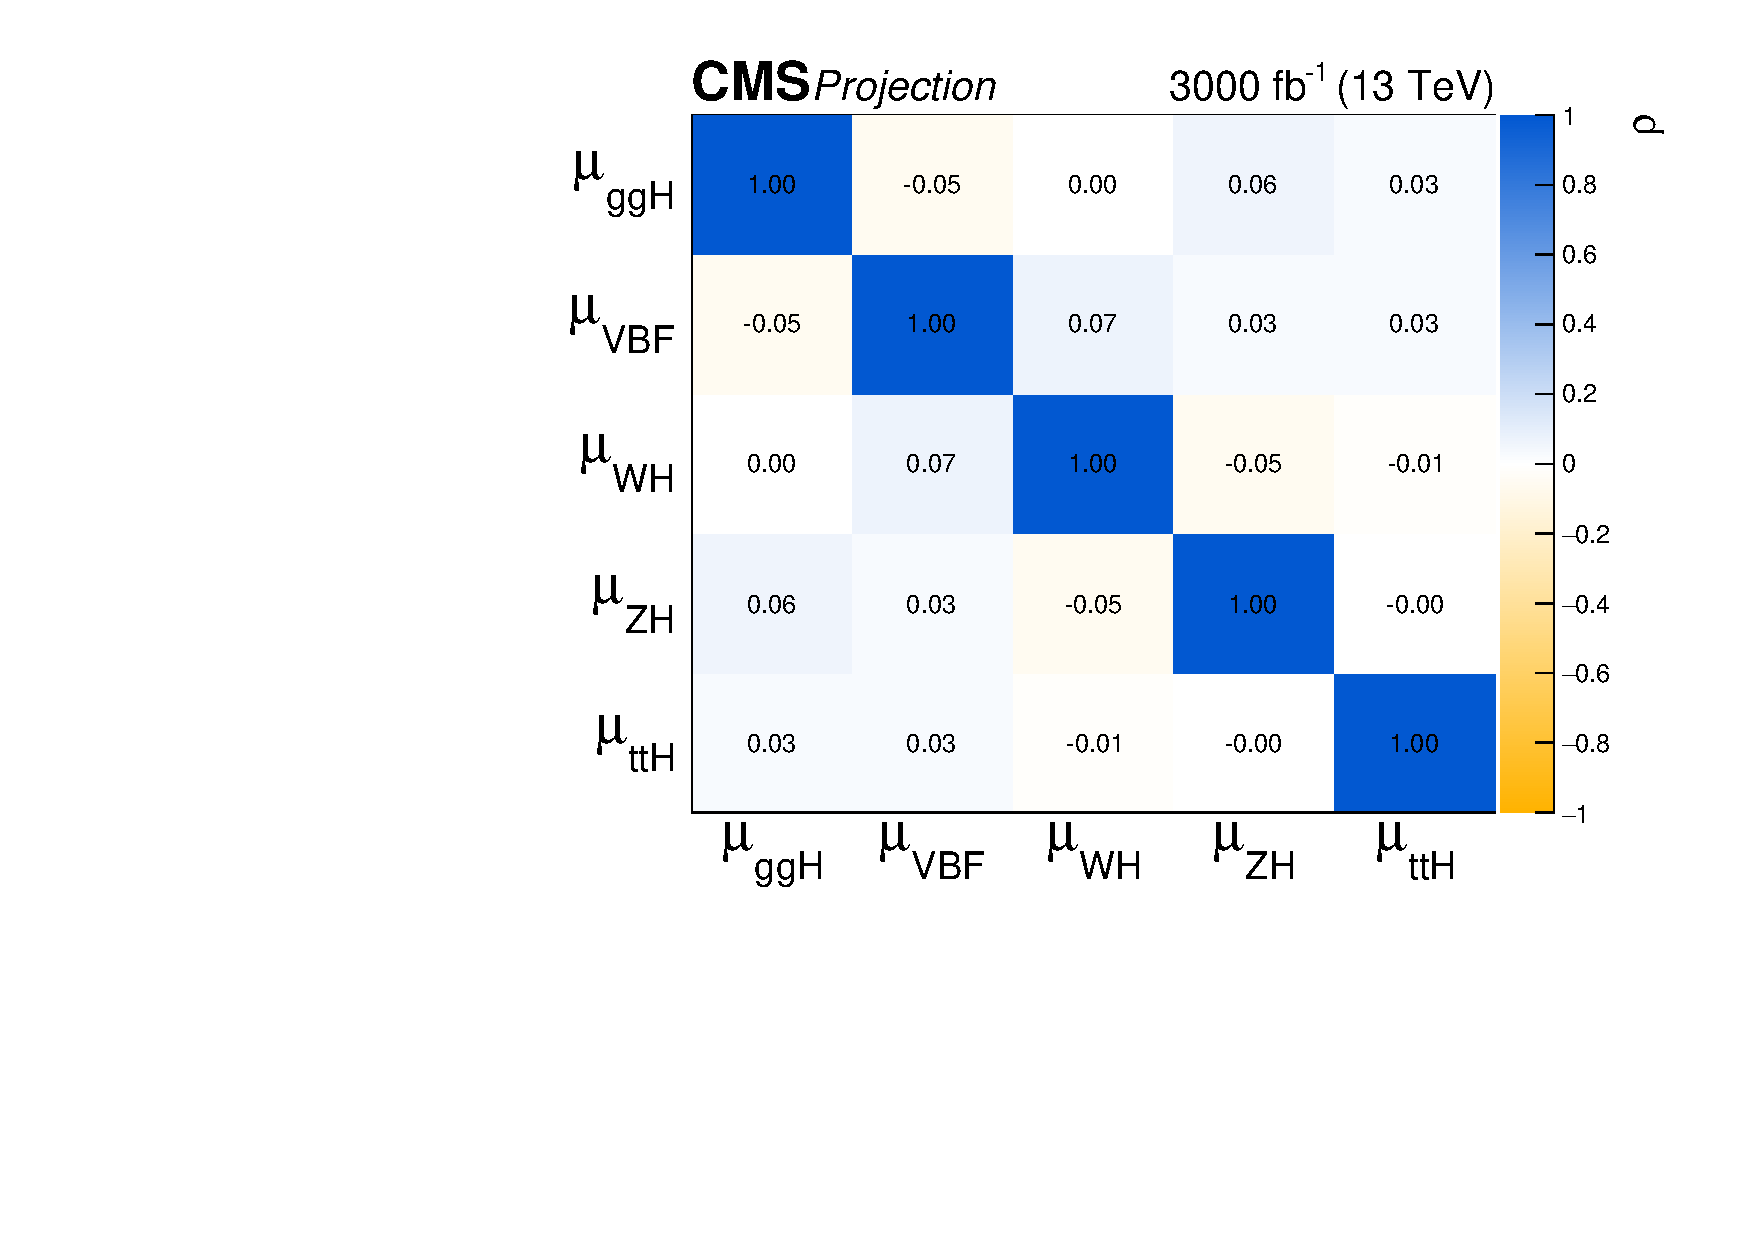
\includegraphics[width=0.48\textwidth]{\main/section2/plots/comb/correlations_A1_5P_S2_3000.pdf}%
%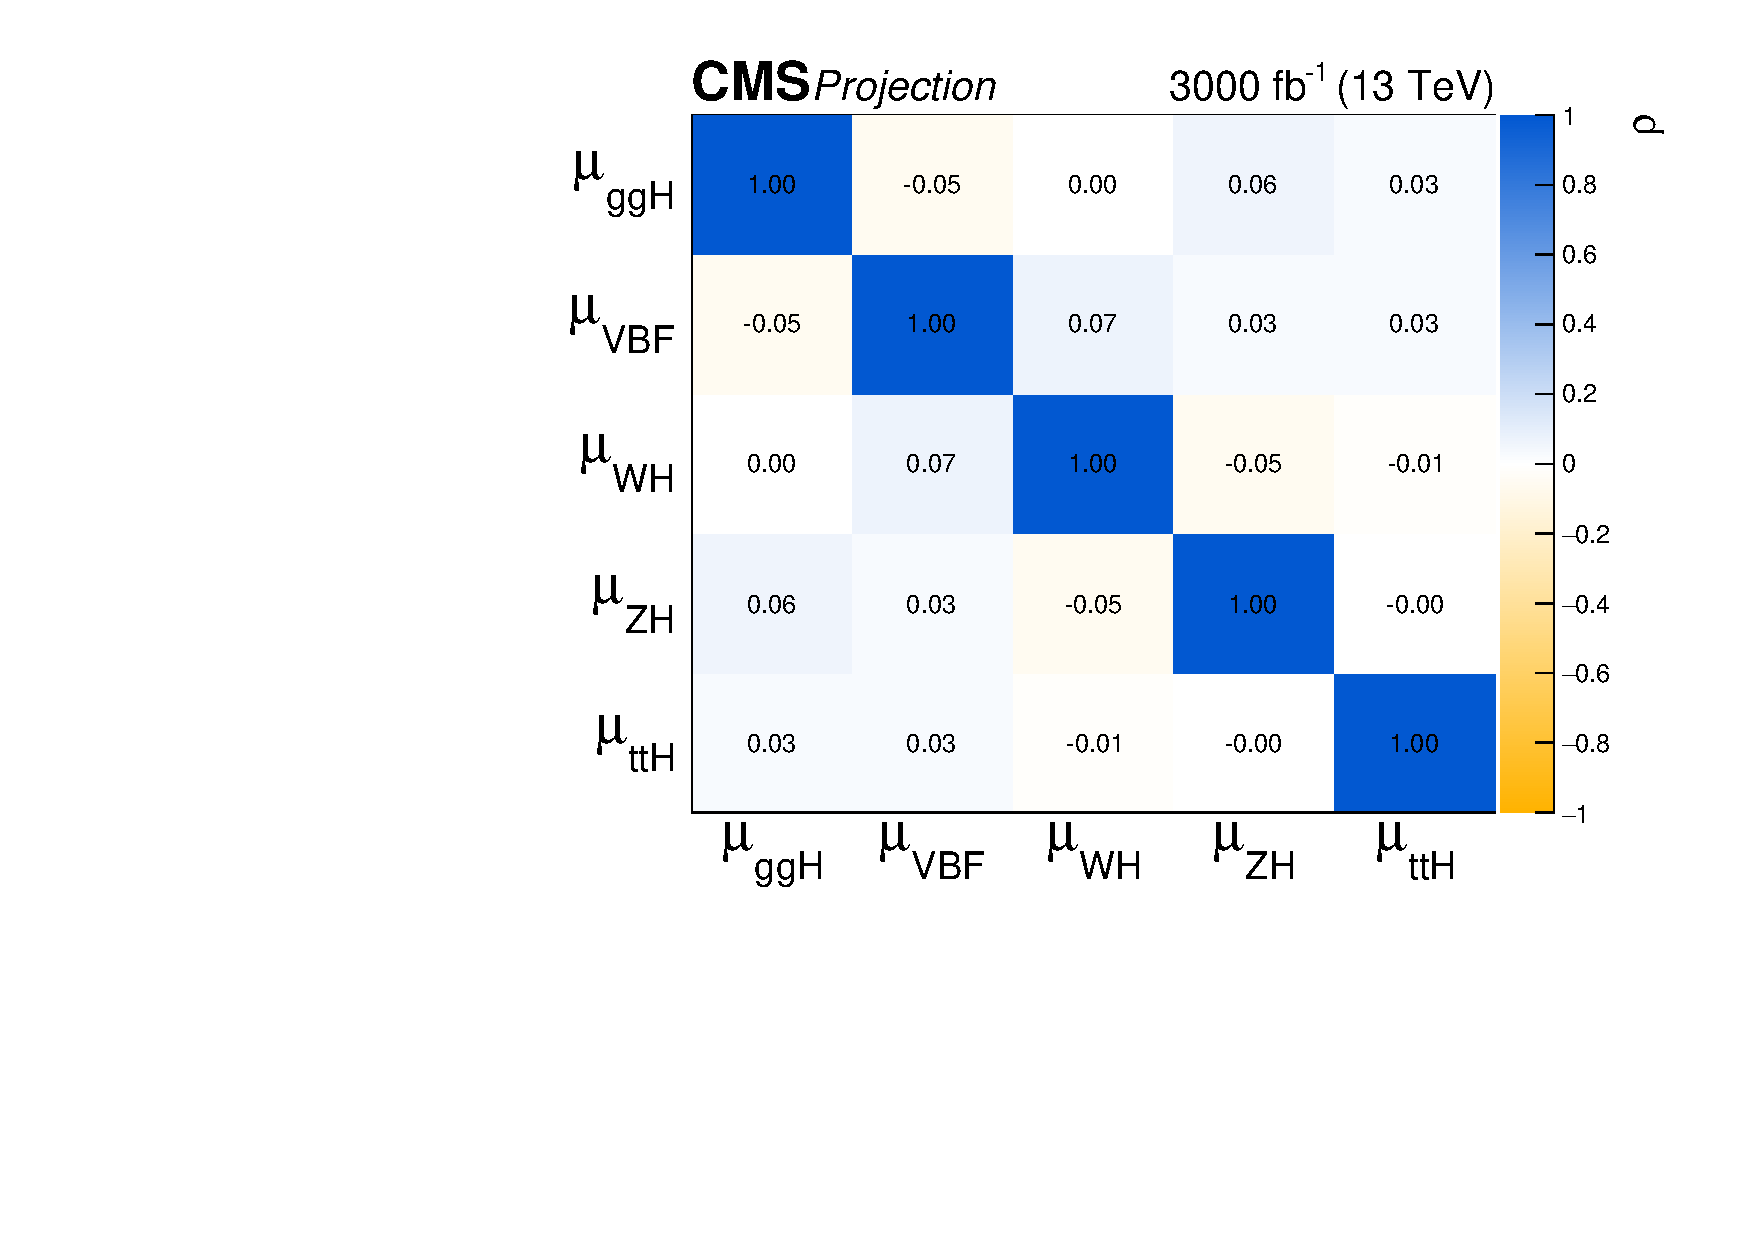
\includegraphics[width=0.48\textwidth]{\main/section2/plots/comb/correlations_A1_5P_S2_3000.pdf}%
%\caption{Correlation coefficients ($\rho$) between the per-production-mode cross sections for S2 (with YR18 systematic uncertainties) for  ATLAS (left) and CMS (right). \wip{add ATLAS results, update all with xsec}}
%\label{fig:corr_A1_5P}
%\end{figure}



%-----------------------------------------------------

\subsubsection{Branching ratios per-decay mode}

The expected $\pm 1\sigma$ uncertainties on the per-decay-mode branching ratios normalised to the SM expectations in S2 for ATLAS, CMS and their combination are summarised in Figure~\ref{fig:summary_A1_5D}.
Additionally, the numerical values for the ATLAS-CMS combination  are also reported in the figure, with the uncertainty decomposed in three components: statistical, experimental and theory.
The S2 uncertainties for the combined ATLAS-CMS extrapolation range from $2-4\%$, with the exception of that on $B^{\mu\mu}$ at $8\%$ and on $B^{Z\gamma}$ at $19\%$.
The numerical values in both S1 and S2 for ATLAS and CMS are given in Table~\ref{tab:summary_A1_5D} where the the breakdown of the uncertainty into four components  is provided. 
In projections of both experiments, the S1 uncertainties are up to a factor of 1.5 larger than those in S2, reflecting the larger systematic component. 
 The systematic uncertainties generally dominate in both S1 and S2. In S2 the signal theory uncertainty is the largest, or joint-largest, component for all parameters except $BR^{\mu\mu}$ and $B^{Z\gamma}$, which remain limited by statistics due to the small  branching fractions. %The $\mu^{\mu\mu}$ uncertainty using the Run~2 dimuon mass resolution instead of the Phase-2 expectation is $14\%$.


\begin{figure}[hbtp]
\centering
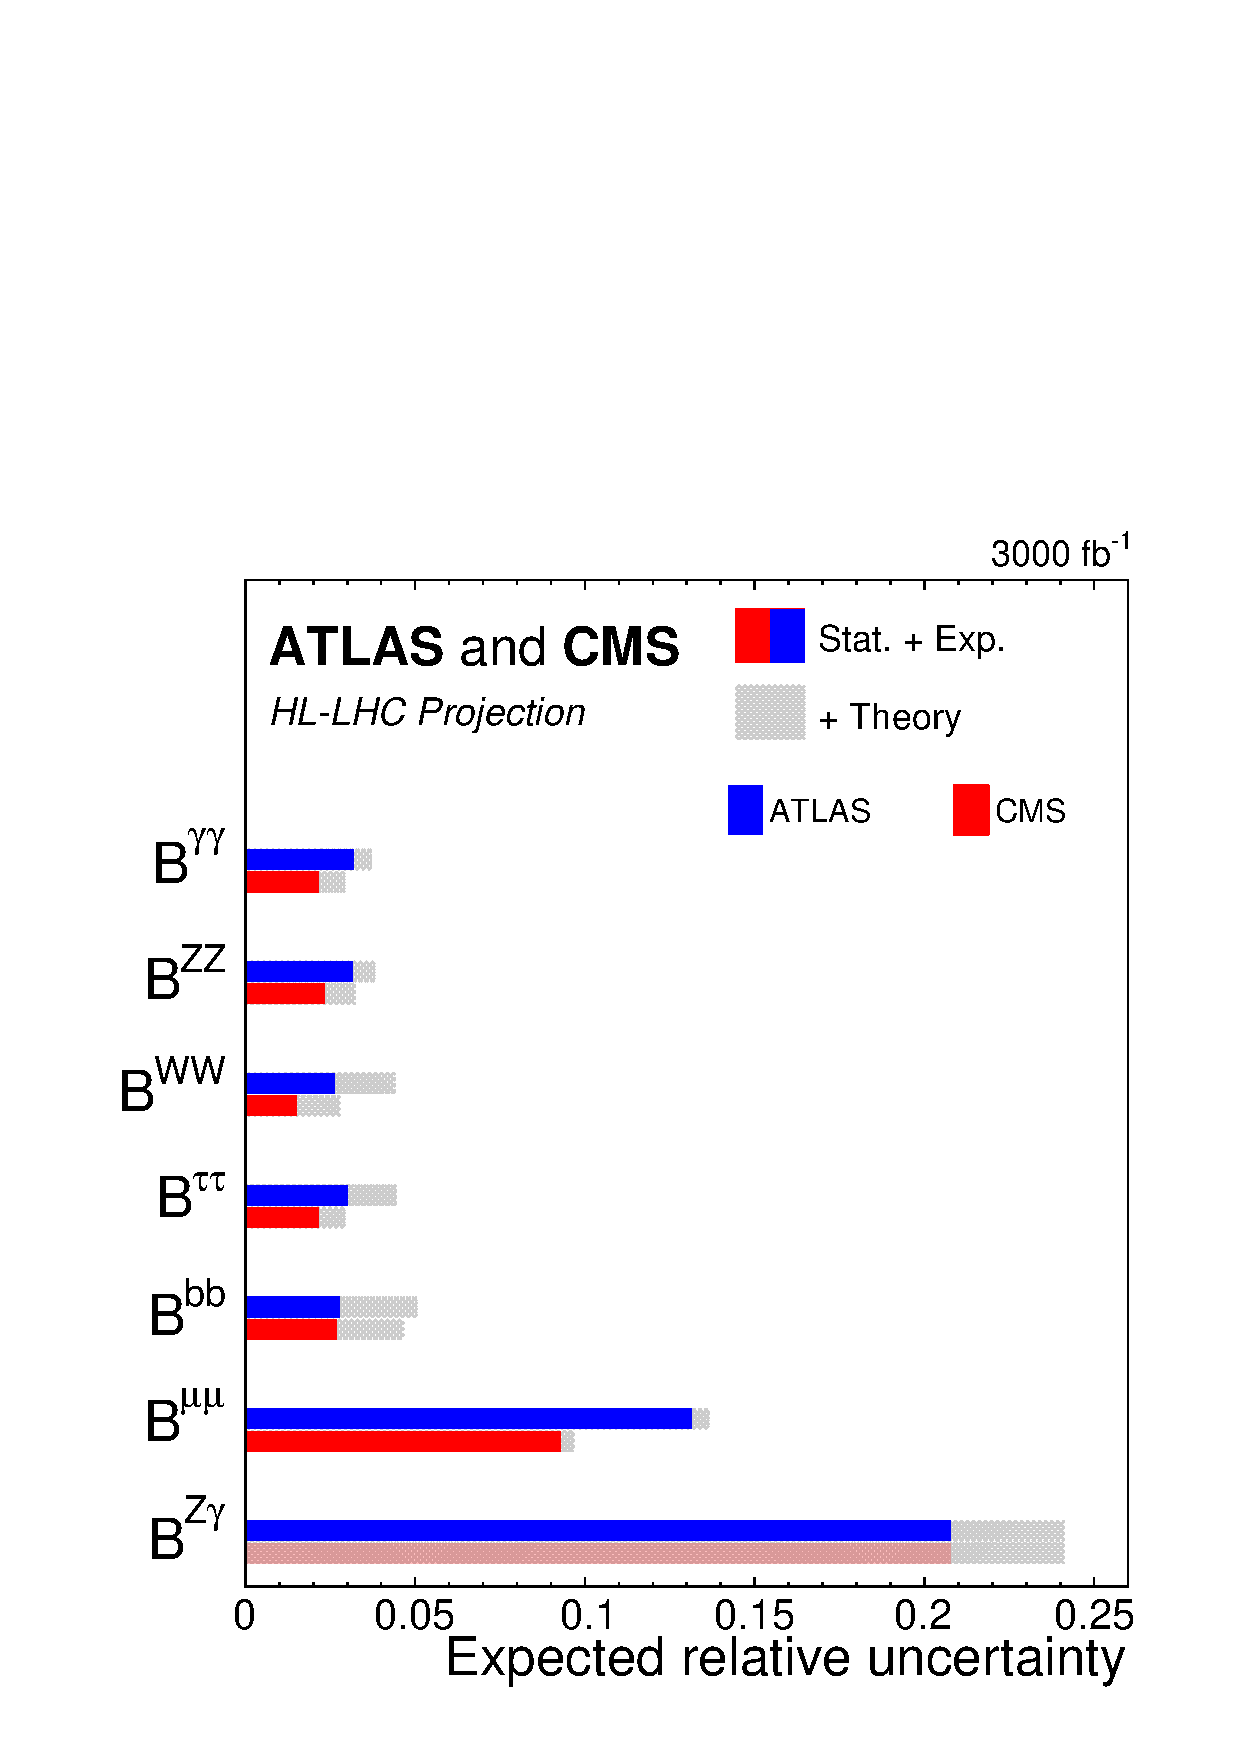
\includegraphics[height=0.332\textheight]{\main/section2/plots/comb/yr_combined_summary_A1_5D_3000.pdf}%
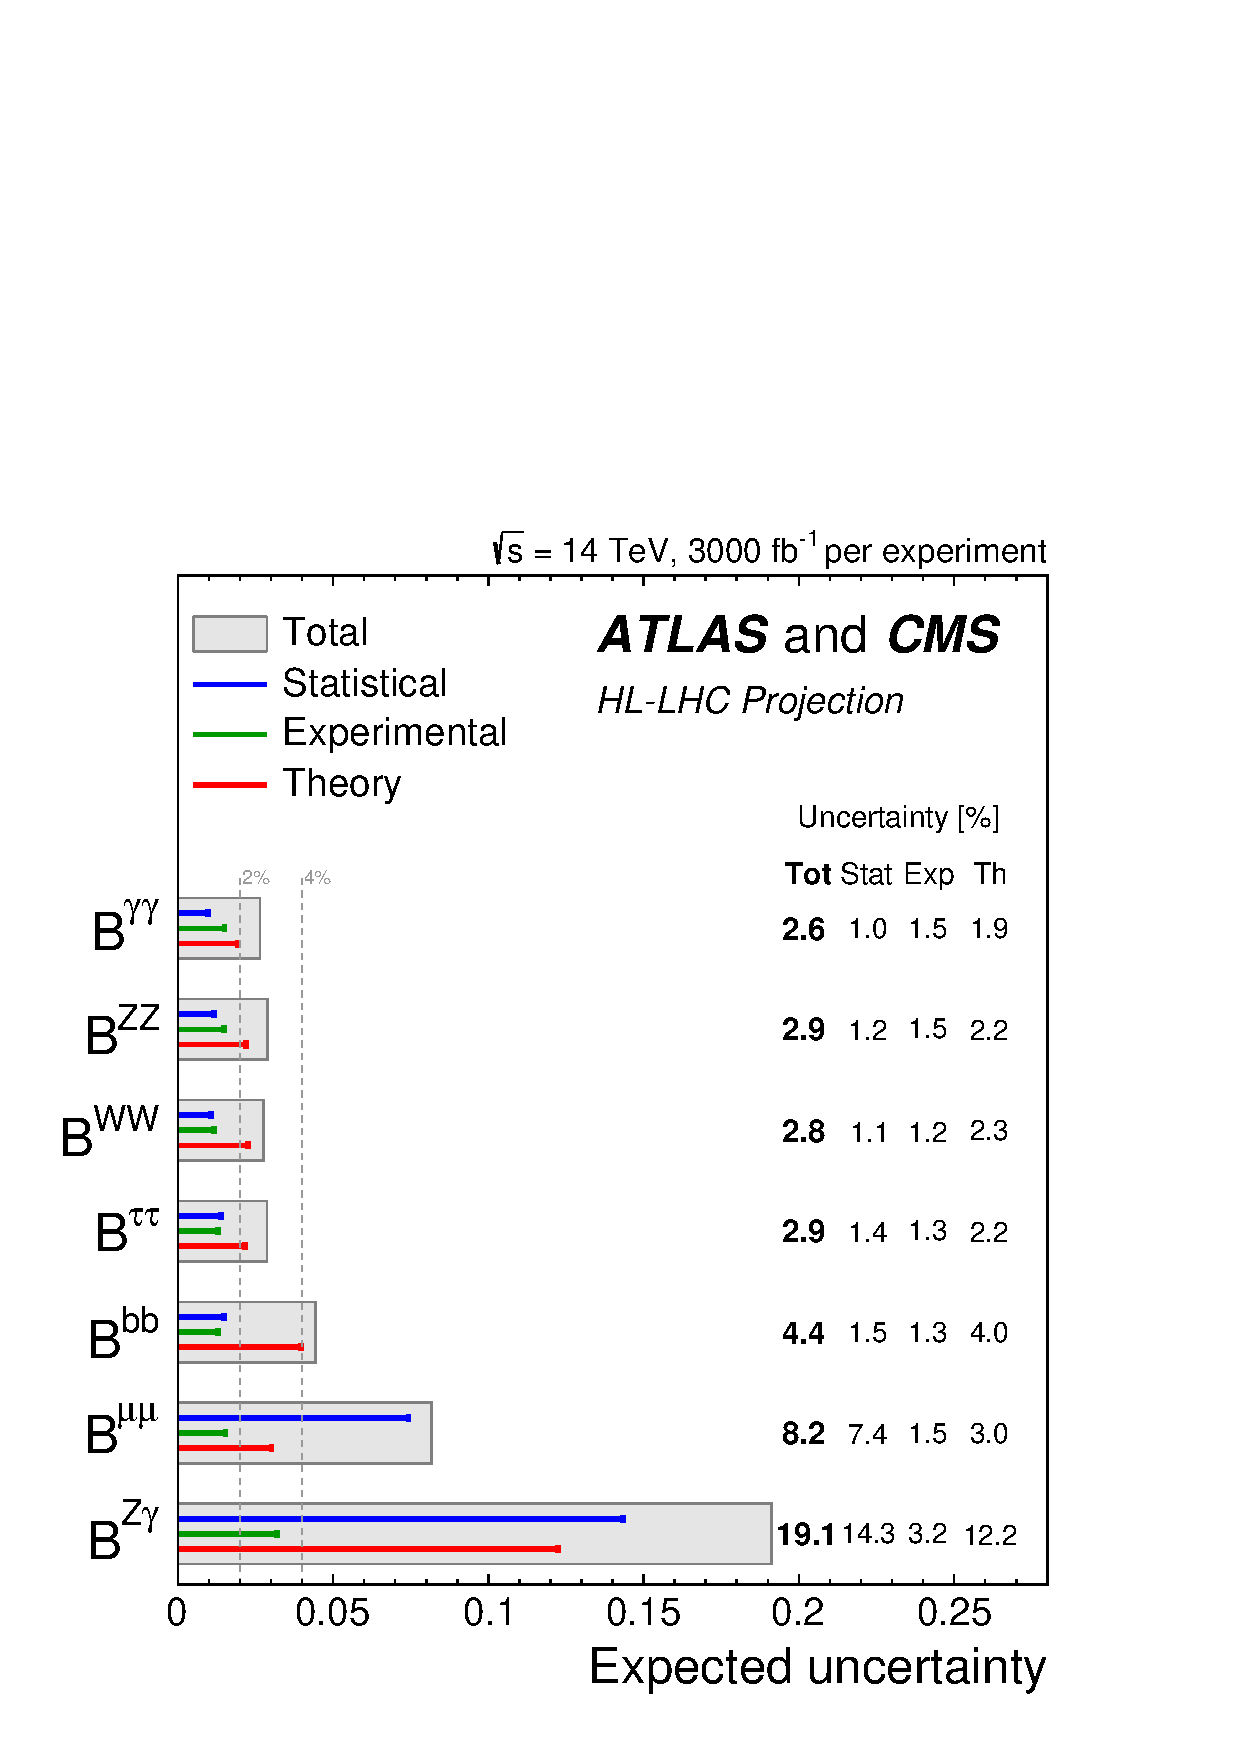
\includegraphics[height=0.33\textheight]{\main/section2/plots/comb/yr_combined_5D.pdf}%
\caption{(left) Summary plot showing the total expected $\pm 1\sigma$ uncertainties in S2 (with YR18 systematic uncertainties) on the  per-decay-mode branching ratios normalised to the SM predictions   for ATLAS (blue)  and CMS (red). The filled coloured box corresponds to the statistical and experimental systematic uncertainties, while the hatched grey area represent the additional contribution to the total uncertainty due to theoretical systematic uncertainties.
(right) Summary plot showing the total expected $\pm 1\sigma$  uncertainties in S2 (with YR18 systematic uncertainties) on the per-decay-mode branching ratios normalised to the SM predictions for the combination of ATLAS and CMS extrapolations. For each measurement,  the total uncertainty is indicated by a grey box while the statistical, experimental and theory uncertainties are indicated by a blue, green and red line respectively. In addition, the numerical values are also reported.}
\label{fig:summary_A1_5D}
\end{figure}


\begin{table}[hbtp]
\centering
\caption{The expected $\pm 1\sigma$ relative uncertainties, expressed as percentages, on the Higgs boson branching ratios normalised by the SM expectations for ATLAS (left) and CMS (right). Values are given for both S1 (with Run~2 systematic uncertainties~\cite{Sirunyan:2018koj}) and S2 (with YR18 systematic uncertainties). The total uncertainty is decomposed into four components: statistical (Stat), signal theory (SigTh), background theory (BkgTh) and experimental (Exp).}
\small
\begin{tabular}{@{} l c c@{\hskip 0.15in} c c c c @{}}
  \hline
   \multicolumn{7}{c}{ATLAS}\\
 \hline  
  &  & \multicolumn{5}{c}{3000 $\text{fb}^{-1}$ uncertainty [\%]} \\
  &  & Total & Stat & Exp & SigTh & BkgTh \\
  \hline
  \multirow{2}{*}{$\mathrm{B}^{\gamma\gamma}$} & S1 &6.0   & 1.2   & 4.7   & 3.4   & 1.3  \\[1pt] 
  & S2  &3.9   & 1.2   & 2.9   & 2.2   & 0.6  \\[4pt]
  \multirow{2}{*}{$\mathrm{B}^{\mathrm{WW}}$} & S1 &6.0   & 1.0   & 2.8   & 4.4   & 2.7  \\[1pt]
  & S2 &4.4   & 1.0   & 2.4   & 3.2   & 1.6  \\[4pt]
  \multirow{2}{*}{$\mathrm{B}^{\mathrm{ZZ}}$} & S1 &5.5   & 1.6   & 3.0   & 4.0   & 1.6  \\[1pt]
  & S2 &3.8   & 1.6   & 2.7   & 1.9   & 0.9  \\[4pt]
  \multirow{2}{*}{$\mathrm{B}^{\mathrm{bb}}$} & S1 &7.6   & 2.0   & 2.4   & 5.0   & 4.8  \\[1pt]
  & S2 &5.0   & 2.0   & 1.9   & 2.8   & 3.2  \\[4pt]
  \multirow{2}{*}{$\mathrm{B}^{\tau\tau }$} & S1 &5.8   & 1.7   & 2.7   & 4.3   & 2.3  \\[1pt]
  & S2 &4.4   & 1.7   & 2.5   & 2.7   & 1.7  \\[4pt]
  \multirow{2}{*}{$\mathrm{B}^{\mu\mu}$} & S1 &14.9  & 12.7  & 3.2   & 6.8   & 0.3  \\[1pt]
  & S2 &13.6  & 12.7  & 3.2   & 3.6   & 0.4  \\[4pt]
  \multirow{2}{*}{$\mathrm{B}^{\mathrm{Z}\gamma}$} & S1 &24.2  & 20.3  & 4.5   & 12.2  & 0.0  \\[1pt]
  & S2 &24.2  & 20.3  & 4.5   & 12.2  & 0.2  \\[4pt]
  \hline
\end{tabular}
\hspace{0.5cm}
\begin{tabular}{@{} l c c@{\hskip 0.15in} c c c c @{}}
 \hline
  &  & \multicolumn{5}{c}{3000 $\text{fb}^{-1}$ uncertainty [\%]} \\
  &  & Total & Stat & Exp & SigTh & BkgTh \\
 \hline
\multirow{2}{*}{$\mathrm{B}^{\gamma\gamma}$} & S1  & 4.4& 1.3 & 2.6 & 3.3 & 0.3  \\[1pt]
                        & S2  & 3.0& 1.3 & 1.7 & 1.9 & 0.3  \\[4pt]
\multirow{2}{*}{$\mathrm{B}^{\mathrm{WW}}$} & S1  & 4.0& 1.0 & 1.4 & 3.5 & 1.0  \\[1pt]
                        & S2  & 2.8& 1.0 & 1.1 & 2.2 & 0.9  \\[4pt]
\multirow{2}{*}{$\mathrm{B}^{\mathrm{ZZ}}$} & S1  & 5.0& 1.6 & 2.5 & 3.5 & 1.9  \\[1pt]
                        & S2  & 3.2& 1.6 & 1.7 & 2.1 & 0.7  \\[4pt]
\multirow{2}{*}{$\mathrm{B}^{\mathrm{bb}}$} & S1  & 7.0& 2.1 & 2.3 & 5.2 & 3.6  \\[1pt]
                        & S2  & 4.7& 2.1 & 1.7 & 2.4 & 2.9  \\[4pt]
\multirow{2}{*}{$\mathrm{B}^{\tau\tau }$} & S1  & 3.9& 1.6 & 1.9 & 2.6 & 1.5  \\[1pt]
                        & S2  & 2.9& 1.6 & 1.4 & 1.9 & 0.6  \\[4pt]
\multirow{2}{*}{$\mathrm{B}^{\mu\mu}$} & S1  & 12.8& 9.1 & 7.6 & 4.7 & 0.8  \\[1pt]
                        & S2  & 9.6& 9.1 & 1.7 & 2.6 & 0.8  \\[4pt]
\hline
\end{tabular}
\label{tab:summary_A1_5D}
\vspace{0.5cm}
\end{table}


 %Figure~\ref{fig:corr_A1_5D} shows the correlation coefficients between the signal strength parameters in S2. 
The correlations range up to 40\%, and are largest between modes where the sensitivity is dominated by gluon-fusion production. This reflects the impact of the theory uncertainties affecting the SM prediction of the gluon-fusion production rate.

%\begin{figure}[hbtp]
%\centering
%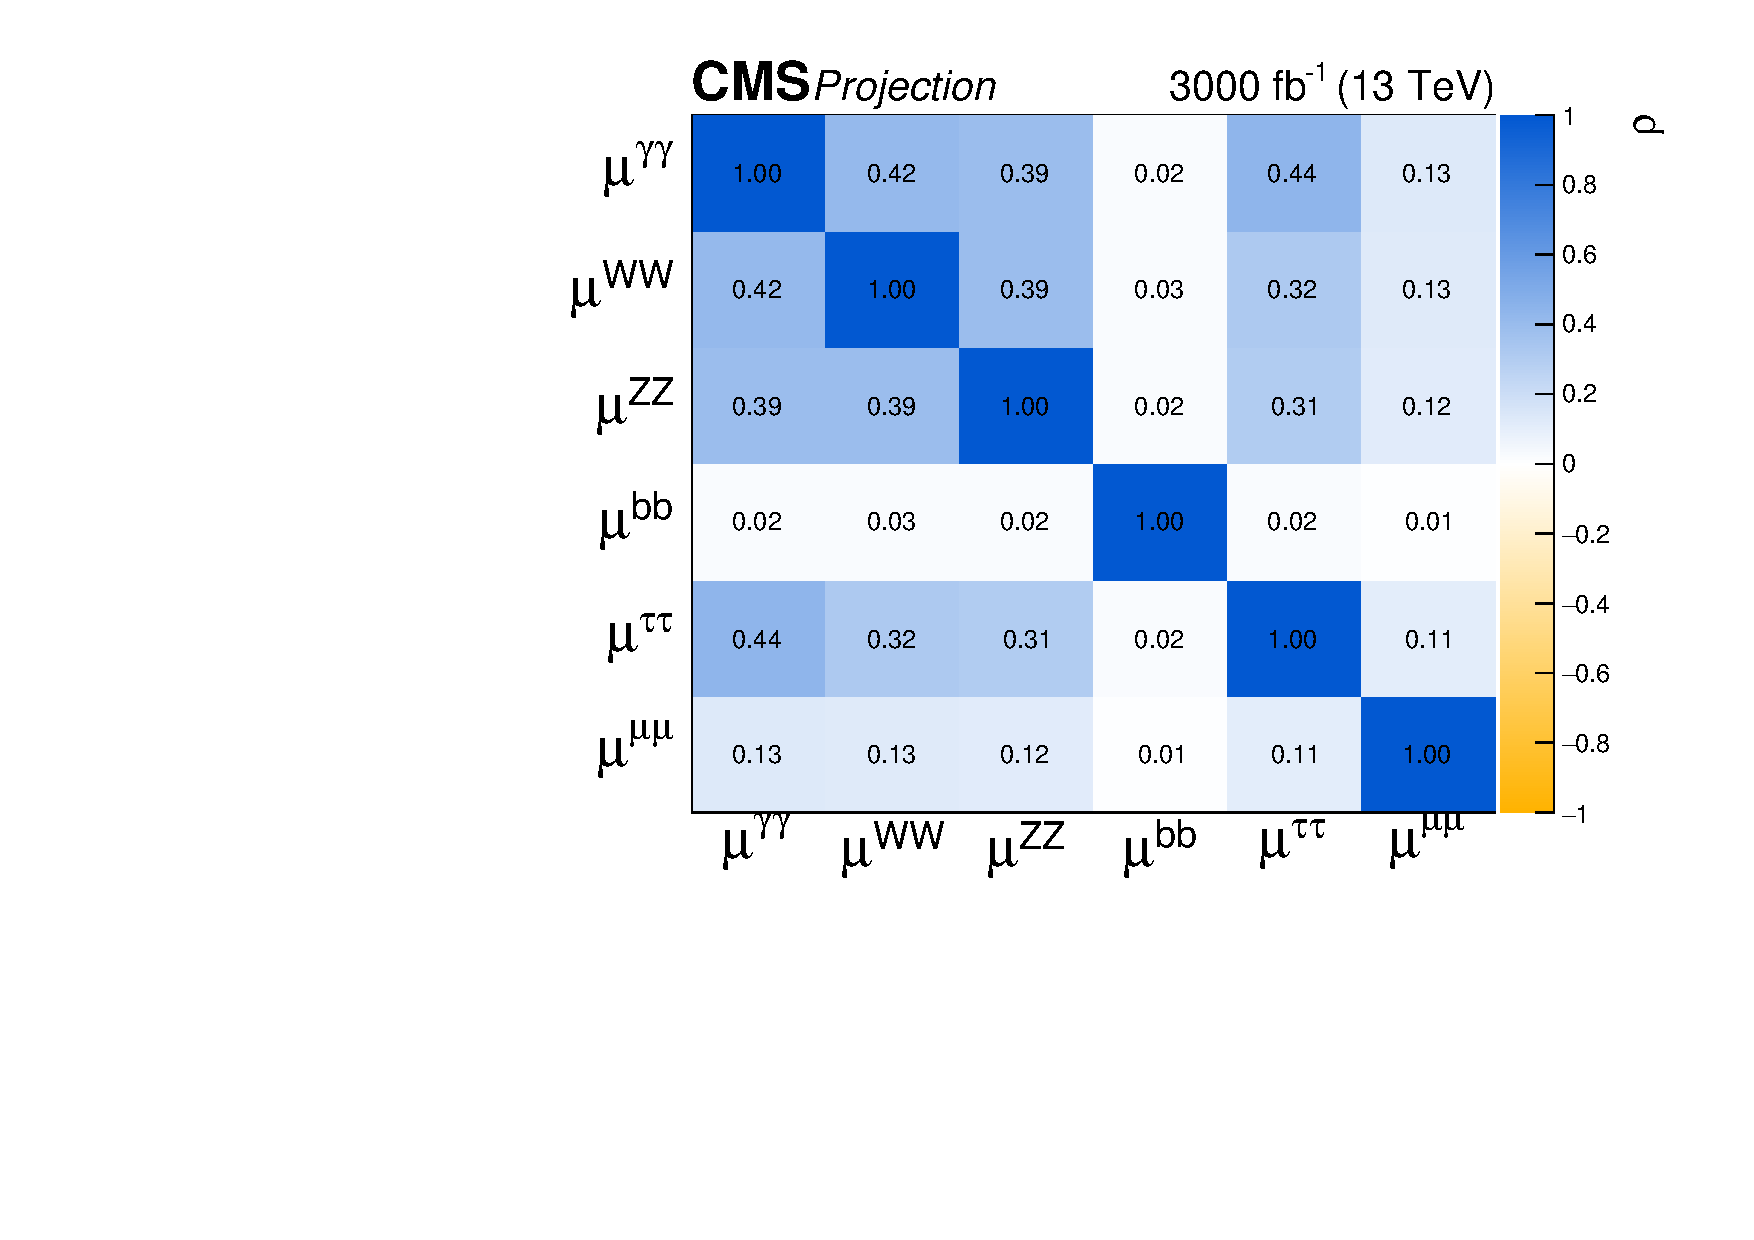
\includegraphics[width=0.48\textwidth]{\main/section2/plots/comb/correlations_A1_5D_S2_3000.pdf}%
%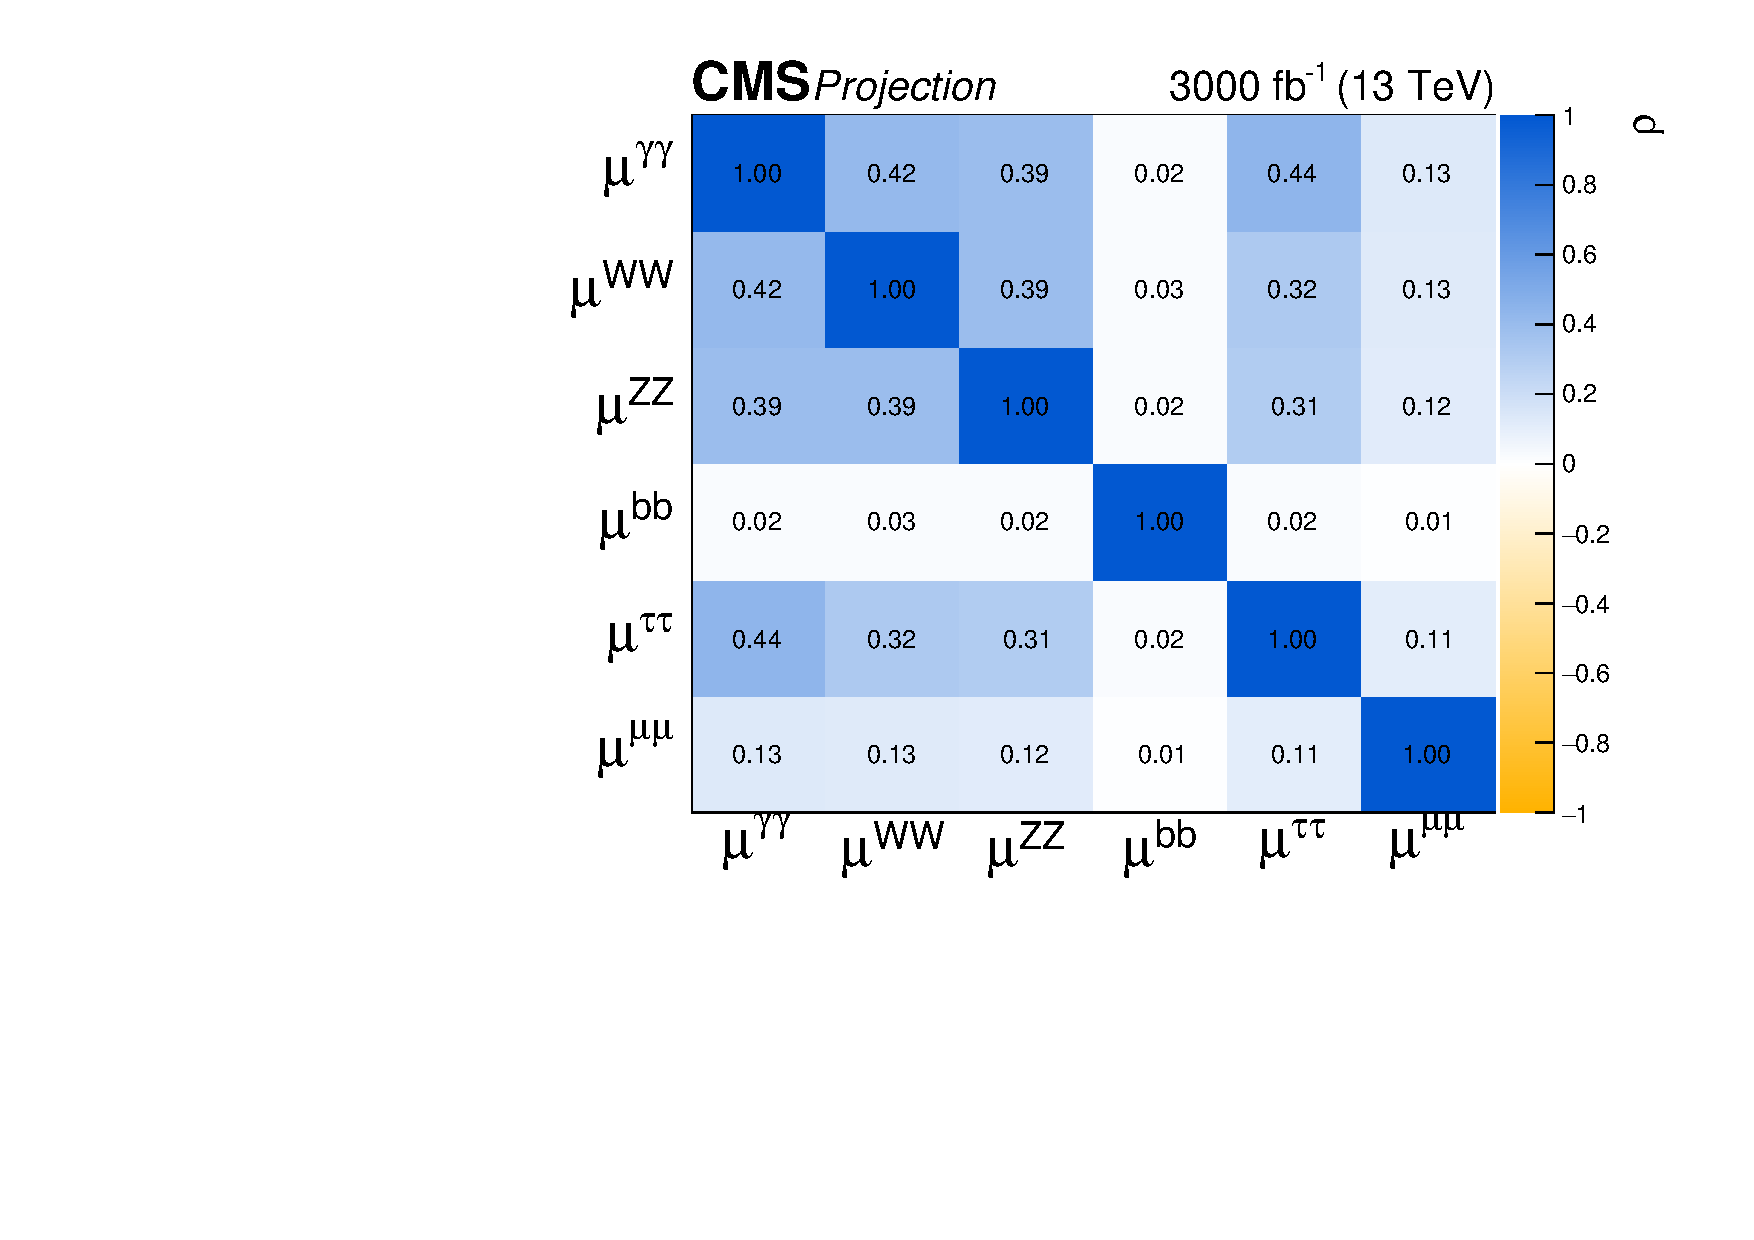
\includegraphics[width=0.48\textwidth]{\main/section2/plots/comb/correlations_A1_5D_S2_3000.pdf}%
%\caption{Correlation coefficients ($\rho$) between the different Higgs boson branching ratios normalized to the SM values for S2 %(with YR18 systematic uncertainties) for ATLAS (left) and CMS (right).\wip{add ATLAS results, move to BR}}
%\label{fig:comb_5D}
%\end{figure}

%\newpage


